\documentclass[
    12pt,
    twoside
]{book}

%\includeonly{chapters/aSecondChapter} % use this command when you only want to compile a small part of the document to check revisions on that file only

% additional latex packages to use
\usepackage{suffix}     % allows to add suffixes when defining commands
\usepackage{xifthen}    % for defining commands with optional arguments in a less opaque way

%%% GEOMETRY %%%%%%%%%%%%%%%%%%%%%%%%%%%%%%%%%%%%%%%%%%%%%%%%%%%%%%%%%%%%%%%%%%%
\usepackage[a4paper, inner=35mm, outer=25mm, top=25mm, bottom=25mm]{geometry}
\usepackage{pdflscape}  % for rotating pages in the PDF so you don't have to crane your neck to read them

%%% TEXT %%%%%%%%%%%%%%%%%%%%%%%%%%%%%%%%%%%%%%%%%%%%%%%%%%%%%%%%%%%%%%%%%%%%%%%
\usepackage{epigraph}   % for ``epigraphs'', i.e. rubrics at the start of chapters
\usepackage{csquotes}   % for fancy display-style quotes
\usepackage{xcolor}     % for changing colour of text, lines etc.
\usepackage{enumitem}   % allows for indented paragraphs within list env.
\setlist{listparindent=\parindent,parsep=0pt}
\usepackage{multicol}   % allows for multiple-columns within list environments

%%% GENERAL FLOATS %%%%%%%%%%%%%%%%%%%%%%%%%%%%%%%%%%%%%%%%%%%%%%%%%%%%%%%%%%%%%
\usepackage{afterpage}

%%% TABLES %%%%%%%%%%%%%%%%%%%%%%%%%%%%%%%%%%%%%%%%%%%%%%%%%%%%%%%%%%%%%%%%%%%%%
\usepackage[flushleft]{threeparttable}  % allows for notes at end of tables
\usepackage{tabularx}   % nice typesetting of tables, including line breaks
    \newcolumntype{L}{>{\raggedright\arraybackslash}X}

%%% GRAPHICS & FIGURES %%%%%%%%%%%%%%%%%%%%%%%%%%%%%%%%%%%%%%%%%%%%%%%%%%%%%%%%%
\usepackage{graphicx}
\graphicspath{ {images/} }
\usepackage{caption}
\usepackage{subcaption} % allows subfigures
\captionsetup{width=.9\textwidth,font=small,labelfont=small}
\captionsetup[subfigure]{justification=justified,singlelinecheck=false}

%%% CHAPTER & TOC SETUP %%%%%%%%%%%%%%%%%%%%%%%%%%%%%%%%%%%%%%%%%%%%%%%%%%%%%%%%
\usepackage{tocbibind}  % for lists in TOC
\usepackage[toc,page]{appendix} % for customizable appendices

\newcounter{lotdepth}   
\setcounter{lotdepth}{3}    % how deep does the list of tables go?

\newcounter{lofdepth}
\setcounter{lofdepth}{3}    % how deep does the list of figures go?

\usepackage{titlesec}
\usepackage{sectsty}    % to change format of all section and chapter headings

\newcommand*{\justifyheading}{\raggedright}

\titleformat    % custom chapter title format
{\chapter} % command
[display] % shape
{\sffamily\bfseries\Huge\justifyheading} % format
{\chaptertitlename \ \thechapter} % label
{0.5ex} % sep
{
    \LARGE
} % before-code
%[] % after-code

\allsectionsfont{\sffamily} % make all headings sans-serif

%%% PAGE SETUP; HEADER & FOOTER %%%%%%%%%%%%%%%%%%%%%%%%%%%%%%%%%%%%%%%%%%%%%%%%
\usepackage{fancyhdr}   % allows fancy formatting of headers & footers
\pagestyle{fancy}
\fancyhf{}
\fancyhead{}    % clear all header fields
\fancyfoot{}    % clear all footer fields
\fancyhead[LE]{\footnotesize\thepage}
\fancyhead[CE]{\footnotesize\selectfont\itshape\nouppercase{\ifnum\value{chapter}>0 \thechapter.~\fi\leftmark}}
\fancyhead[CO]{\footnotesize\selectfont\itshape\nouppercase{\ifnum\value{chapter}>0 \thechapter.~\fi\leftmark}}
\fancyhead[RO]{\footnotesize\thepage}
\renewcommand{\headrulewidth}{0pt}      % Line at the header invisible
\renewcommand{\footrulewidth}{0pt}      % Line at the footer invisible

\renewcommand{\chaptermark}[1]{\markboth{#1}{}}

\fancypagestyle{plain}{ % used for e.g. chapter title pages
    \fancyhf{}
    \fancyhead{}    % clear all header fields
    \fancyfoot{}    % clear all footer fields
    \fancyfoot[C]{\thepage}
    \renewcommand{\headrulewidth}{0pt}  % Line at the header invisible
    \renewcommand{\footrulewidth}{0pt}  % Line at the footer invisible
}

\fancypagestyle{frontAndBack}{ % for front and back matter
    \fancyhf{}
    \fancyhead{}    % clear all header fields
    \fancyfoot{}    % clear all footer fields
    \fancyhead[LE]{\footnotesize\thepage}
    \fancyhead[CE]{\footnotesize\selectfont\itshape\nouppercase{\ifnum\value{chapter}>0 \thechapter.~\fi\leftmark}}
    \fancyhead[CO]{\footnotesize\selectfont\itshape\nouppercase{\ifnum\value{chapter}>0 \thechapter.~\fi\leftmark}}
    \fancyhead[RO]{\footnotesize\thepage}
    \renewcommand{\headrulewidth}{0pt}      % Line at the header invisible
    \renewcommand{\footrulewidth}{0pt}      % Line at the footer invisible
}

\fancypagestyle{main}{ % for main matter (and appendices)
    \fancyhf{}
    \fancyhead{}    % clear all header fields
    \fancyfoot{}    % clear all footer fields
    \fancyhead[LE]{\footnotesize\thepage}
    \fancyhead[CE]{\footnotesize\selectfont\itshape\nouppercase{\ifnum\value{chapter}>0 \thechapter.~\fi\leftmark}}
    \fancyhead[CO]{\footnotesize\selectfont\itshape\nouppercase{\ifnum\value{chapter}>0 \thechapter.~\fi\leftmark}}
    \fancyhead[RO]{\footnotesize\thepage}
    \renewcommand{\headrulewidth}{0pt}      % Line at the header invisible
    \renewcommand{\footrulewidth}{0pt}      % Line at the footer invisible
}

%%% LINE SPACING %%%%%%%%%%%%%%%%%%%%%%%%%%%%%%%%%%%%%%%%%%%%%%%%%%%%%%%%%%%%%%%
\usepackage{setspace}
\setstretch{1.25}

%%% BIBLIOGRAPHY %%%%%%%%%%%%%%%%%%%%%%%%%%%%%%%%%%%%%%%%%%%%%%%%%%%%%%%%%%%%%%%
\usepackage[
    backref=true, 
    backend=biber, 
    bibencoding=utf8, 
    style=authoryear-comp, 
    maxcitenames=2, 
    uniquelist=false, 
    sorting=nyt,
    url=false,
    eprint=false,
    isbn=false,
    giveninits=true,
    uniquename=init
]{biblatex} % uniquelist=false means e.g. Siebesma et al. (2004) and Siebesma et
% al. (2007) do not have unique cite keys despite having different author lists;
% backref adds ref. in bib to page(s) cited in text
\renewbibmacro{in:}{
    \ifentrytype{article}{}{
        \printtext{\bibstring{in}\intitlepunct}
    }
} % don't print "in" for articles
\renewcommand*{\bibfont}{\small}

\AtEveryBibitem{
    \clearfield{day}
    \clearfield{month}
}   % stop superfluous fields from appearing

\DefineBibliographyStrings{english}{%
  backrefpage = {cit. on p.},% originally "cited on page"
  backrefpages = {cit. on pp.},% originally "cited on pages"
}

%%% REVIEW & EDITING %%%%%%%%%%%%%%%%%%%%%%%%%%%%%%%%%%%%%%%%%%%%%%%%%%%%%%%%%%%
\newboolean{draft}
\setboolean{draft}{true} % set to false in main doc preamble if you don't want annotations/to-do notes to appear
\usepackage{ulem} % required for strikethrough text
\normalem % use normal italics for emphasis rather than underline

% Display with annotation if draft == True; without annotation if False
\newcommand{\add}[1]{%
    \ifthenelse{ \boolean{draft} }%
    {\textcolor{blue}{#1}}%
    {\unskip#1}%
}
\newcommand{\delete}[1]{%
    \ifthenelse{ \boolean{draft} }%
    {\textcolor{red}{\textit{\sout{#1}}}}%
    {\unskip}%
}
\newcommand{\edit}[2]{%
    \ifthenelse{ \boolean{draft} }%
    {\textcolor{red}{\textit{\sout{#1}}} \textcolor{blue}{#2}}%
    {\unskip#2}%
}
\newcommand{\note}[1]{%
    \ifthenelse{ \boolean{draft} }%
    {\textcolor{red}{\textbf{#1}}}%
    {\unskip}%
}
\newcommand{\todonote}[1]{%
    \ifthenelse{ \boolean{draft} }%
    {\textcolor{red}{\textbf{[To-do: #1]}}}%
    {\unskip}%
}

%%% MATHEMATICS %%%%%%%%%%%%%%%%%%%%%%%%%%%%%%%%%%%%%%%%%%%%%%%%%%%%%%%%%%%%%%%%
%%% MATHS ENV. STUFF %%%%%%%%%%%%%%%%%%%%%%%%%%%%%%%%%%%%%%%%%%%%%%%%%%%%%%%%%%%
%%% PACKAGES
\usepackage{mathtools}
\usepackage{amsmath}
\usepackage{amssymb}
\usepackage{amsthm} % for theorem environments
\usepackage{amsfonts}   % specifically for blackboard bold
\usepackage{physics}    % package full of pre-defined physics notation, e.g. \abs and \norm for absolute value and norm, \vdot for vector dot product, \dv{}{} for derivatives, and \bra \ket \braket etc.
\usepackage{cancel} % for nice cancelling out of terms in equations

%%% COMMANDS
%% Note: some of these commands require the ifthen and/or suffix packages
% set {...}
\newcommand{\set}[1]{ \ensuremath{ \left\{ #1 \right\} } }
% ``Big Oh''
\newcommand{\bigOh}[1]{ \ensuremath{ \mathcal{O}\left( #1 \right) } }
% vector
\renewcommand{\vec}[1]{\ensuremath{\boldsymbol{\mathbf{#1}}}}
% vector \ell
\newcommand{\vecEll}{\ensuremath{\boldsymbol\ell}}
% unit vector
\newcommand{\unit}[1]{\ensuremath{\hat{\vec{#1}}}}
% nice version of measure dx for integrals
\newcommand{\diff}[2][]{%
    \ifthenelse{ \isempty{#1} }
        {\ensuremath{\operatorname{d}\!{#2}}}
        {\ensuremath{\operatorname{d}^{#1}\!{#2}}}
}
% horizontal divergence
\newcommand{\divH}[1]{\ensuremath{\boldsymbol{\nabla}_\text{H}\mathbin{\vdot} #1}}
% tensor
\newcommand{\tensor}[1]{\ensuremath{\boldsymbol{\mathsf{#1}}}}
% tensor parts
\newcommand{\iso}{\ensuremath{\tensor{iso}}}
\newcommand{\dev}{\ensuremath{\tensor{dev}}}
\newcommand{\symm}{\ensuremath{\tensor{symm}}}
\newcommand{\asymm}{\ensuremath{\tensor{asymm}}}
% double-colon contraction notation
\newcommand{\contract}{\ensuremath{\mathbin{\boldsymbol{:}}}}
% trace
\renewcommand{\tr}{\ensuremath{\tensor{tr}}}
% tensor identity
\newcommand{\ident}[1][]{%
    \ifthenelse{ \isempty{#1} }
        {\ensuremath{\tensor{I}}}
        {\ensuremath{\tensor{I}}_{#1}}
}
% transpose
\newcommand*{\trans}{\ensuremath{^{\mathsf{T}}}}
% big-D material derivative
\newcommand{\Dv}[2]{\ensuremath{\frac{\operatorname{D}\!{#1}}{\operatorname{D}\!{#2}}}}
\WithSuffix\newcommand\Dv*[2]{\ensuremath{\flatfrac{\operatorname{D}\!{#1}}{\operatorname{D}\!{#2}}}}
% multi-fluid material derivative
\newcommand{\DvMF}[3]{\ensuremath{\frac{\operatorname{D}_{#1}\!{#2}}{\operatorname{D}\!{#3}}}}
\WithSuffix\newcommand\DvMF*[3]{\ensuremath{\flatfrac{\operatorname{D}_{#1}\!{#2}}{\operatorname{D}\!{#3}}}}
% Laplacian and divergence commands consistent with \grad
\renewcommand{\laplacian}{\grad^2}
\newcommand{\laplaciantilde}{\widetilde{\grad}^2}
\newcommand{\laplacianhat}{\widehat{\grad}^2}
\newcommand{\divtilde}[1]{\widetilde{\grad}\mathbin{\vdot}{#1}}
\newcommand{\divhat}[1]{\widehat{\grad}\mathbin{\vdot}{#1}}
% nice filtering operator
\newcommand{\filter}[2][]{%
    \ifthenelse{ \isempty{#1} }
        {\ensuremath{ \left\langle {#2} \right\rangle }}
        {\ensuremath{ \left\langle {#2} \right\rangle_{#1} }}
}
% nice Reynolds averaging operator
\newcommand{\reynolds}[1]{%
        {\ensuremath{ \left\langle {#1} \right\rangle_{\mathrm{R}} }}
}
% resolved and subfilter parts
\newcommand{\resolved}[2][]{%
    \ifthenelse{ \isempty{#1} }
        {\ensuremath{ {#2}^\mathrm{r} }}
        {\ensuremath{ {#2}_{#1}^\mathrm{r} }}
}
\newcommand{\subfilter}[2][]{%
    \ifthenelse{ \isempty{#1} }
        {\ensuremath{ {#2}^\mathrm{s} }}
        {\ensuremath{ {#2}_{#1}^\mathrm{s} }}
}
\newcommand{\favreResolved}[2][]{%
    \ifthenelse{ \isempty{#1} }
        {\ensuremath{ \widetilde{#2}^\mathrm{r} }}
        {\ensuremath{ \widetilde{#2}_{#1}^\mathrm{r} }}
}
\newcommand{\favreSubfilter}[2][]{%
    \ifthenelse{ \isempty{#1} }
        {\ensuremath{ \widetilde{#2}^\mathrm{r} }}
        {\ensuremath{ \widetilde{#2}_{#1}^\mathrm{r} }}
}
% dimensionless groups for fluid dynamics
\renewcommand{\Re}{\ensuremath{\operatorname{Re}}}  % Reynolds number
\renewcommand{\Pr}{\ensuremath{\operatorname{Pr}}}  % Prandtl number
\newcommand{\Ra}{\ensuremath{\operatorname{Ra}}}    % Rayleigh number
\newcommand{\Nu}{\ensuremath{\operatorname{Nu}}}    % Nusselt number
\newcommand{\Co}{\ensuremath{\operatorname{Co}}}    % Courant number
\newcommand{\Fr}{\ensuremath{\operatorname{Fr}}}    % Froude number
\newcommand{\Ro}{\ensuremath{\operatorname{Ro}}}    % Rossby number

%%% THEOREM, REMARK, ASSUMPTION ETC. ENVIRONMENTS %%%%%%%%%%%%%%%%%%%%%%%%%%%%%%
\theoremstyle{definition}
\newtheorem{assumption}{Assumption}
\newtheorem{definition}{Definition}
\newtheorem*{conjecture}{Conjecture}
\theoremstyle{plain}
\newtheorem*{aside}{Aside}

%%% MISC. %%%%%%%%%%%%%%%%%%%%%%%%%%%%%%%%%%%%%%%%%%%%%%%%%%%%%%%%%%%%%%%%%%%%%%
% allow display equation environments to break over page breaks
\allowdisplaybreaks

%%% REFERENCES, URLS & HYPERLINKING %%%%%%%%%%%%%%%%%%%%%%%%%%%%%%%%%%%%%%%%%%%%
\PassOptionsToPackage{hyphens}{url}\usepackage{hyperref}   % everyone says to include hyperref last...
\hypersetup{
    colorlinks=false
}   % colour links looked pretty horrible...
\usepackage{xurl} % for nice line-breaks in URLs
\usepackage[capitalise,noabbrev]{cleveref}   % nice automatic typesetting of e.g. theorem, chapter etc. references
\AtBeginEnvironment{appendices}{\crefalias{chapter}{appendix}} % change chapter to section if you want within-chapter appendices

\graphicspath{ {book/images/} }
\addbibresource{book/miniBib.bib}

%%% VERSION CONTROL %%%%%%%%%%%%%%%%%%%%%%%%%%%%%%%%%%%%%%%%%%%%%%%%%%%%%%%%%%%%
\usepackage[mark,local]{gitinfo2}
\renewcommand{\gitMark}{
    %This version: \gitBranch\,@\,\gitAbbrevHash{} \textbullet{} \gitAuthorDate
    This version: gitBranch\,@\,gitHash \textbullet{} D.~Shipley \textbullet{} 22--09--1401
}
% you can change this to say whatever you like; unfortunately the gitinfo2 package doesn't really work with Overleaf, so if you're using Overleaf and want git-related versioning in the watermark, you'll have to either type the commit IDs etc. in manually, or add the gitHeadInfo.gin file (generated from some local copy of the git repo) into your Overleaf document tree and use the "local" option when loading gitinfo2
% remove [mark] from the package inclusion statement if you don't want the watermark to appear

%%% TEXT TO ONLY APPEAR IN DRAFTS %%%%%%%%%%%%%%%%%%%%%%%%%%%%%%%%%%%%%%%%%%%%%%
\setboolean{draft}{true}    % set to false if you don't want annotations/to-do notes to appear

%%% NONSENSE TEXT FOR THIS MWE ONLY %%%%%%%%%%%%%%%%%%%%%%%%%%%%%%%%%%%%%%%%%%%%
\usepackage{blindtext}

%%%%%%%%%%%%%%%%%%%%%%%%%%%%%%%%%%%%%%%%%%%%%%%%%%%%%%%%%%%%%%%%%%%%%%%%%%%%%%%%
%%% BEGIN MAIN DOCUMENT %%%%%%%%%%%%%%%%%%%%%%%%%%%%%%%%%%%%%%%%%%%%%%%%%%%%%%%%
%%%%%%%%%%%%%%%%%%%%%%%%%%%%%%%%%%%%%%%%%%%%%%%%%%%%%%%%%%%%%%%%%%%%%%%%%%%%%%%%

\begin{document}

% front matter
\frontmatter
\pagestyle{frontAndBack}

\begin{titlepage}
    \begin{center}
        \vspace*{2em}
        
        \Huge
        \textbf{A custom \LaTeX\ macro for theses \& books}
        
        \vspace{5em}
        
        
\includegraphics[width=0.2\textwidth]{universityOfReading_shieldLogo.png}
        
        \vspace{3em}
              
        \LARGE
        Dan Shipley
        
        \vspace{0.5em}
        
        \large
        Department of Meteorology\\
        \vspace{0.5em}
        University of Reading\\
        
        \vspace{6em}
        
        A thesis presented for the degree of\\
        \vspace{0.5em}
        \emph{Doctor of Philosophy}\\
        \vspace{0.7em}
        September 2022
        
    \end{center}
\end{titlepage}

\thispagestyle{empty}
\begin{center}
    This revision: \texttt{\gitBranch\,@\,\gitAbbrevHash}.

    Version number: \gitRel
\end{center}


\vspace{2em}
\noindent\textit{\color{red}
    Add whatever you like here, or delete entirely. 
    Works best with the gitInfo2 package, but alas that doesn't play nicely with Overleaf.
}

\thispagestyle{empty}
\vspace*{\stretch{1}}
\begin{center}
    \textit{For\textellipsis?}
\end{center}
\vspace{\stretch{2}} % space below dedication is twice the space above
\cleardoublepage

\renewcommand*{\justifyheading}{\centering} % centred headings for this bit
\chapter{Declaration}

I confirm that this is my own work and the use of all material from other sources has been properly and fully acknowledged.

\vspace{2em}

\hfill \textit{Your Name} \hspace{1em}

\chapter{Acknowledgements}

Something soppy (and likely long-winded) goes here.

\chapter{Abstract}

This document is a minimal working example (MWE) to demonstrate the style, as well as some of the functionality, of Dan Shipley's \LaTeX\ book macro.
So far this has only been used for his thesis \parencite{phd:Shipley2021} and some postdoc notes.
Textbook on fluid dynamics coming in 2040\textellipsis

The MWE includes all of the front matter etc. required of a thesis at the University of Reading.
These can of course be deleted/altered if the desired document is not such a thesis.

\renewcommand*{\justifyheading}{\raggedright} % back to left-aligned ragged-right headings

\listoffigures

\listoftables

\chapter{A Note on Notation}

It is my firm belief that every text making heavy use of mathematics owes to its readers a glossary of terms and notation, \textit{especially} where that notation is unusual (or where multiple conventions currently coexist).
Whether this should be placed in the front matter or the end matter, and whether the note takes the form of a descriptive dictionary, a succinct table, some of both, or something else entirely, is up to the writer.

\begin{table}[h]
    \centering
    \begin{tabularx}{\textwidth}{ l | L }
        \hline
        Notation    & Description   \\
        \hline
        $\varphi$               & A generic flow variable, assumed $\varphi(\vec{x},t)$ \\
        $\filter[g]{\varphi}$   & Spatial filter of variable $\varphi$ with respect to the kernel $g$  \\
        $\resolved{\varphi}$    & Resolved part of variable $\varphi$                   \\
        $\subfilter{\varphi}$   & Subfilter part of variable $\varphi$                  \\
        $I_i$                   & Indicator function of partition $i$                   \\
        $\resolved[i]{\varphi}$ & Resolved part of variable $\varphi$ in partition $i$  \\
        $\subfilter[i]{\varphi}$& Subfilter part of variable $\varphi$ in partition $i$ \\
        $s(a,b)$                & Generalized centred second moment of variables $a,b$  \\
        $a$                     & A scalar                                              \\
        $\vec{a}$               & A vector (components $a_\mu$)                         \\
        $\tensor{a}$            & A tensor (components $a_{\mu\nu}$)                    \\
        $\ident[d]$             & $d$-dimensional identity tensor                       \\
        $\mathbb{R}$            & The real numbers                                      \\
        $\in$                   & Set inclusion, i.e. $a \in S$ means ``$a$ is a member of the set $S$''    \\
        $\mathcal{O}$           & ``Big Oh'' asymptotic order notation                  \\
        \hline
    \end{tabularx}
    %\label{tab:my_label}
\end{table}

\tableofcontents

\pagestyle{empty}

\renewcommand{\epigraphflush}{center}
\vspace*{60mm}
\epigraph{I accept clouds exist.}{Peter A. Clark, 2018\nocite{pcomm:ClarkClouds2018}}

\cleardoublepage

% main chapters
\mainmatter
\pagestyle{main}

\chapter{Overview}\label{ch:intro}

Here I give an overview of the basic functionality of the macro.
Firstly, a few words about the overall look of the ``book'' macro: I like sans-serif headings; line-spacing slightly wider than the \LaTeX\ default; page numbers in the corners of the header, chapter titles in the centre of the header, leaving ample room for footnotes/version information at the bottom of the page.
If your preferences differ, these things may be changed in the \texttt{CHAPTER \& TOC SETUP}, \texttt{HEADER \& FOOTER}, and \texttt{LINE SPACING} sections of \texttt{dansBookMacro}.

\section{How to construct a book/thesis in \LaTeX}

This document is a (fairly) minimal working example of how to construct a book-length document in \LaTeX\ using \texttt{dansBookMacro}.
The essential components are as follows:
\begin{enumerate}
    \item Preamble
    \begin{enumerate}
        \item Define document class (book; 12pt, twoside).
        \item \verb!% additional latex packages to use
\usepackage{suffix}     % allows to add suffixes when defining commands
\usepackage{xifthen}    % for defining commands with optional arguments in a less opaque way

%%% GEOMETRY %%%%%%%%%%%%%%%%%%%%%%%%%%%%%%%%%%%%%%%%%%%%%%%%%%%%%%%%%%%%%%%%%%%
\usepackage[a4paper, inner=35mm, outer=25mm, top=25mm, bottom=25mm]{geometry}
\usepackage{pdflscape}  % for rotating pages in the PDF so you don't have to crane your neck to read them

%%% TEXT %%%%%%%%%%%%%%%%%%%%%%%%%%%%%%%%%%%%%%%%%%%%%%%%%%%%%%%%%%%%%%%%%%%%%%%
\usepackage{epigraph}   % for ``epigraphs'', i.e. rubrics at the start of chapters
\usepackage{csquotes}   % for fancy display-style quotes
\usepackage{xcolor}     % for changing colour of text, lines etc.
\usepackage{enumitem}   % allows for indented paragraphs within list env.
\setlist{listparindent=\parindent,parsep=0pt}
\usepackage{multicol}   % allows for multiple-columns within list environments

%%% GENERAL FLOATS %%%%%%%%%%%%%%%%%%%%%%%%%%%%%%%%%%%%%%%%%%%%%%%%%%%%%%%%%%%%%
\usepackage{afterpage}

%%% TABLES %%%%%%%%%%%%%%%%%%%%%%%%%%%%%%%%%%%%%%%%%%%%%%%%%%%%%%%%%%%%%%%%%%%%%
\usepackage[flushleft]{threeparttable}  % allows for notes at end of tables
\usepackage{tabularx}   % nice typesetting of tables, including line breaks
    \newcolumntype{L}{>{\raggedright\arraybackslash}X}

%%% GRAPHICS & FIGURES %%%%%%%%%%%%%%%%%%%%%%%%%%%%%%%%%%%%%%%%%%%%%%%%%%%%%%%%%
\usepackage{graphicx}
\graphicspath{ {images/} }
\usepackage{caption}
\usepackage{subcaption} % allows subfigures
\captionsetup{width=.9\textwidth,font=small,labelfont=small}
\captionsetup[subfigure]{justification=justified,singlelinecheck=false}

%%% CHAPTER & TOC SETUP %%%%%%%%%%%%%%%%%%%%%%%%%%%%%%%%%%%%%%%%%%%%%%%%%%%%%%%%
\usepackage{tocbibind}  % for lists in TOC
\usepackage[toc,page]{appendix} % for customizable appendices

\newcounter{lotdepth}   
\setcounter{lotdepth}{3}    % how deep does the list of tables go?

\newcounter{lofdepth}
\setcounter{lofdepth}{3}    % how deep does the list of figures go?

\usepackage{titlesec}
\usepackage{sectsty}    % to change format of all section and chapter headings

\newcommand*{\justifyheading}{\raggedright}

\titleformat    % custom chapter title format
{\chapter} % command
[display] % shape
{\sffamily\bfseries\Huge\justifyheading} % format
{\chaptertitlename \ \thechapter} % label
{0.5ex} % sep
{
    \LARGE
} % before-code
%[] % after-code

\allsectionsfont{\sffamily} % make all headings sans-serif

%%% PAGE SETUP; HEADER & FOOTER %%%%%%%%%%%%%%%%%%%%%%%%%%%%%%%%%%%%%%%%%%%%%%%%
\usepackage{fancyhdr}   % allows fancy formatting of headers & footers
\pagestyle{fancy}
\fancyhf{}
\fancyhead{}    % clear all header fields
\fancyfoot{}    % clear all footer fields
\fancyhead[LE]{\footnotesize\thepage}
\fancyhead[CE]{\footnotesize\selectfont\itshape\nouppercase{\ifnum\value{chapter}>0 \thechapter.~\fi\leftmark}}
\fancyhead[CO]{\footnotesize\selectfont\itshape\nouppercase{\ifnum\value{chapter}>0 \thechapter.~\fi\leftmark}}
\fancyhead[RO]{\footnotesize\thepage}
\renewcommand{\headrulewidth}{0pt}      % Line at the header invisible
\renewcommand{\footrulewidth}{0pt}      % Line at the footer invisible

\renewcommand{\chaptermark}[1]{\markboth{#1}{}}

\fancypagestyle{plain}{ % used for e.g. chapter title pages
    \fancyhf{}
    \fancyhead{}    % clear all header fields
    \fancyfoot{}    % clear all footer fields
    \fancyfoot[C]{\thepage}
    \renewcommand{\headrulewidth}{0pt}  % Line at the header invisible
    \renewcommand{\footrulewidth}{0pt}  % Line at the footer invisible
}

\fancypagestyle{frontAndBack}{ % for front and back matter
    \fancyhf{}
    \fancyhead{}    % clear all header fields
    \fancyfoot{}    % clear all footer fields
    \fancyhead[LE]{\footnotesize\thepage}
    \fancyhead[CE]{\footnotesize\selectfont\itshape\nouppercase{\ifnum\value{chapter}>0 \thechapter.~\fi\leftmark}}
    \fancyhead[CO]{\footnotesize\selectfont\itshape\nouppercase{\ifnum\value{chapter}>0 \thechapter.~\fi\leftmark}}
    \fancyhead[RO]{\footnotesize\thepage}
    \renewcommand{\headrulewidth}{0pt}      % Line at the header invisible
    \renewcommand{\footrulewidth}{0pt}      % Line at the footer invisible
}

\fancypagestyle{main}{ % for main matter (and appendices)
    \fancyhf{}
    \fancyhead{}    % clear all header fields
    \fancyfoot{}    % clear all footer fields
    \fancyhead[LE]{\footnotesize\thepage}
    \fancyhead[CE]{\footnotesize\selectfont\itshape\nouppercase{\ifnum\value{chapter}>0 \thechapter.~\fi\leftmark}}
    \fancyhead[CO]{\footnotesize\selectfont\itshape\nouppercase{\ifnum\value{chapter}>0 \thechapter.~\fi\leftmark}}
    \fancyhead[RO]{\footnotesize\thepage}
    \renewcommand{\headrulewidth}{0pt}      % Line at the header invisible
    \renewcommand{\footrulewidth}{0pt}      % Line at the footer invisible
}

%%% LINE SPACING %%%%%%%%%%%%%%%%%%%%%%%%%%%%%%%%%%%%%%%%%%%%%%%%%%%%%%%%%%%%%%%
\usepackage{setspace}
\setstretch{1.25}

%%% BIBLIOGRAPHY %%%%%%%%%%%%%%%%%%%%%%%%%%%%%%%%%%%%%%%%%%%%%%%%%%%%%%%%%%%%%%%
\usepackage[
    backref=true, 
    backend=biber, 
    bibencoding=utf8, 
    style=authoryear-comp, 
    maxcitenames=2, 
    uniquelist=false, 
    sorting=nyt,
    url=false,
    eprint=false,
    isbn=false,
    giveninits=true,
    uniquename=init
]{biblatex} % uniquelist=false means e.g. Siebesma et al. (2004) and Siebesma et
% al. (2007) do not have unique cite keys despite having different author lists;
% backref adds ref. in bib to page(s) cited in text
\renewbibmacro{in:}{
    \ifentrytype{article}{}{
        \printtext{\bibstring{in}\intitlepunct}
    }
} % don't print "in" for articles
\renewcommand*{\bibfont}{\small}

\AtEveryBibitem{
    \clearfield{day}
    \clearfield{month}
}   % stop superfluous fields from appearing

\DefineBibliographyStrings{english}{%
  backrefpage = {cit. on p.},% originally "cited on page"
  backrefpages = {cit. on pp.},% originally "cited on pages"
}

%%% REVIEW & EDITING %%%%%%%%%%%%%%%%%%%%%%%%%%%%%%%%%%%%%%%%%%%%%%%%%%%%%%%%%%%
\newboolean{draft}
\setboolean{draft}{true} % set to false in main doc preamble if you don't want annotations/to-do notes to appear
\usepackage{ulem} % required for strikethrough text
\normalem % use normal italics for emphasis rather than underline

% Display with annotation if draft == True; without annotation if False
\newcommand{\add}[1]{%
    \ifthenelse{ \boolean{draft} }%
    {\textcolor{blue}{#1}}%
    {\unskip#1}%
}
\newcommand{\delete}[1]{%
    \ifthenelse{ \boolean{draft} }%
    {\textcolor{red}{\textit{\sout{#1}}}}%
    {\unskip}%
}
\newcommand{\edit}[2]{%
    \ifthenelse{ \boolean{draft} }%
    {\textcolor{red}{\textit{\sout{#1}}} \textcolor{blue}{#2}}%
    {\unskip#2}%
}
\newcommand{\note}[1]{%
    \ifthenelse{ \boolean{draft} }%
    {\textcolor{red}{\textbf{#1}}}%
    {\unskip}%
}
\newcommand{\todonote}[1]{%
    \ifthenelse{ \boolean{draft} }%
    {\textcolor{red}{\textbf{[To-do: #1]}}}%
    {\unskip}%
}

%%% MATHEMATICS %%%%%%%%%%%%%%%%%%%%%%%%%%%%%%%%%%%%%%%%%%%%%%%%%%%%%%%%%%%%%%%%
%%% MATHS ENV. STUFF %%%%%%%%%%%%%%%%%%%%%%%%%%%%%%%%%%%%%%%%%%%%%%%%%%%%%%%%%%%
%%% PACKAGES
\usepackage{mathtools}
\usepackage{amsmath}
\usepackage{amssymb}
\usepackage{amsthm} % for theorem environments
\usepackage{amsfonts}   % specifically for blackboard bold
\usepackage{physics}    % package full of pre-defined physics notation, e.g. \abs and \norm for absolute value and norm, \vdot for vector dot product, \dv{}{} for derivatives, and \bra \ket \braket etc.
\usepackage{cancel} % for nice cancelling out of terms in equations

%%% COMMANDS
%% Note: some of these commands require the ifthen and/or suffix packages
% set {...}
\newcommand{\set}[1]{ \ensuremath{ \left\{ #1 \right\} } }
% ``Big Oh''
\newcommand{\bigOh}[1]{ \ensuremath{ \mathcal{O}\left( #1 \right) } }
% vector
\renewcommand{\vec}[1]{\ensuremath{\boldsymbol{\mathbf{#1}}}}
% vector \ell
\newcommand{\vecEll}{\ensuremath{\boldsymbol\ell}}
% unit vector
\newcommand{\unit}[1]{\ensuremath{\hat{\vec{#1}}}}
% nice version of measure dx for integrals
\newcommand{\diff}[2][]{%
    \ifthenelse{ \isempty{#1} }
        {\ensuremath{\operatorname{d}\!{#2}}}
        {\ensuremath{\operatorname{d}^{#1}\!{#2}}}
}
% horizontal divergence
\newcommand{\divH}[1]{\ensuremath{\boldsymbol{\nabla}_\text{H}\mathbin{\vdot} #1}}
% tensor
\newcommand{\tensor}[1]{\ensuremath{\boldsymbol{\mathsf{#1}}}}
% tensor parts
\newcommand{\iso}{\ensuremath{\tensor{iso}}}
\newcommand{\dev}{\ensuremath{\tensor{dev}}}
\newcommand{\symm}{\ensuremath{\tensor{symm}}}
\newcommand{\asymm}{\ensuremath{\tensor{asymm}}}
% double-colon contraction notation
\newcommand{\contract}{\ensuremath{\mathbin{\boldsymbol{:}}}}
% trace
\renewcommand{\tr}{\ensuremath{\tensor{tr}}}
% tensor identity
\newcommand{\ident}[1][]{%
    \ifthenelse{ \isempty{#1} }
        {\ensuremath{\tensor{I}}}
        {\ensuremath{\tensor{I}}_{#1}}
}
% transpose
\newcommand*{\trans}{\ensuremath{^{\mathsf{T}}}}
% big-D material derivative
\newcommand{\Dv}[2]{\ensuremath{\frac{\operatorname{D}\!{#1}}{\operatorname{D}\!{#2}}}}
\WithSuffix\newcommand\Dv*[2]{\ensuremath{\flatfrac{\operatorname{D}\!{#1}}{\operatorname{D}\!{#2}}}}
% multi-fluid material derivative
\newcommand{\DvMF}[3]{\ensuremath{\frac{\operatorname{D}_{#1}\!{#2}}{\operatorname{D}\!{#3}}}}
\WithSuffix\newcommand\DvMF*[3]{\ensuremath{\flatfrac{\operatorname{D}_{#1}\!{#2}}{\operatorname{D}\!{#3}}}}
% Laplacian and divergence commands consistent with \grad
\renewcommand{\laplacian}{\grad^2}
\newcommand{\laplaciantilde}{\widetilde{\grad}^2}
\newcommand{\laplacianhat}{\widehat{\grad}^2}
\newcommand{\divtilde}[1]{\widetilde{\grad}\mathbin{\vdot}{#1}}
\newcommand{\divhat}[1]{\widehat{\grad}\mathbin{\vdot}{#1}}
% nice filtering operator
\newcommand{\filter}[2][]{%
    \ifthenelse{ \isempty{#1} }
        {\ensuremath{ \left\langle {#2} \right\rangle }}
        {\ensuremath{ \left\langle {#2} \right\rangle_{#1} }}
}
% nice Reynolds averaging operator
\newcommand{\reynolds}[1]{%
        {\ensuremath{ \left\langle {#1} \right\rangle_{\mathrm{R}} }}
}
% resolved and subfilter parts
\newcommand{\resolved}[2][]{%
    \ifthenelse{ \isempty{#1} }
        {\ensuremath{ {#2}^\mathrm{r} }}
        {\ensuremath{ {#2}_{#1}^\mathrm{r} }}
}
\newcommand{\subfilter}[2][]{%
    \ifthenelse{ \isempty{#1} }
        {\ensuremath{ {#2}^\mathrm{s} }}
        {\ensuremath{ {#2}_{#1}^\mathrm{s} }}
}
\newcommand{\favreResolved}[2][]{%
    \ifthenelse{ \isempty{#1} }
        {\ensuremath{ \widetilde{#2}^\mathrm{r} }}
        {\ensuremath{ \widetilde{#2}_{#1}^\mathrm{r} }}
}
\newcommand{\favreSubfilter}[2][]{%
    \ifthenelse{ \isempty{#1} }
        {\ensuremath{ \widetilde{#2}^\mathrm{r} }}
        {\ensuremath{ \widetilde{#2}_{#1}^\mathrm{r} }}
}
% dimensionless groups for fluid dynamics
\renewcommand{\Re}{\ensuremath{\operatorname{Re}}}  % Reynolds number
\renewcommand{\Pr}{\ensuremath{\operatorname{Pr}}}  % Prandtl number
\newcommand{\Ra}{\ensuremath{\operatorname{Ra}}}    % Rayleigh number
\newcommand{\Nu}{\ensuremath{\operatorname{Nu}}}    % Nusselt number
\newcommand{\Co}{\ensuremath{\operatorname{Co}}}    % Courant number
\newcommand{\Fr}{\ensuremath{\operatorname{Fr}}}    % Froude number
\newcommand{\Ro}{\ensuremath{\operatorname{Ro}}}    % Rossby number

%%% THEOREM, REMARK, ASSUMPTION ETC. ENVIRONMENTS %%%%%%%%%%%%%%%%%%%%%%%%%%%%%%
\theoremstyle{definition}
\newtheorem{assumption}{Assumption}
\newtheorem{definition}{Definition}
\newtheorem*{conjecture}{Conjecture}
\theoremstyle{plain}
\newtheorem*{aside}{Aside}

%%% MISC. %%%%%%%%%%%%%%%%%%%%%%%%%%%%%%%%%%%%%%%%%%%%%%%%%%%%%%%%%%%%%%%%%%%%%%
% allow display equation environments to break over page breaks
\allowdisplaybreaks

%%% REFERENCES, URLS & HYPERLINKING %%%%%%%%%%%%%%%%%%%%%%%%%%%%%%%%%%%%%%%%%%%%
\PassOptionsToPackage{hyphens}{url}\usepackage{hyperref}   % everyone says to include hyperref last...
\hypersetup{
    colorlinks=false
}   % colour links looked pretty horrible...
\usepackage{xurl} % for nice line-breaks in URLs
\usepackage[capitalise,noabbrev]{cleveref}   % nice automatic typesetting of e.g. theorem, chapter etc. references
\AtBeginEnvironment{appendices}{\crefalias{chapter}{appendix}} % change chapter to section if you want within-chapter appendices!.
        \item Re-define any geometry commands you like here; for instance, the standard setup has unequal inner and outer margins (respectively 35mm and 25mm), intended to allow room for binding the printed version.
        However a PDF-only copy should have equal margins; the command \verb!\geometry{margin=30mm}! alters this without changing any of the page numbering or typesetting etc.
        \item Set graphics path and bib file.
        \item Set up version control watermarking.
        \item Declare draft status (default: \texttt{true}).
    \end{enumerate}
    \item Front matter
    \begin{enumerate}
        \item The start of the front matter is demarcated by the \verb!\frontmatter! command; among other things, this causes page numbering to use Roman numerals.
        \item I have defined a custom page style for the front and back matter, activated here by the command \verb!\pagestyle{frontAndBack}!.
        This is editable in the \texttt{PAGE SETUP; HEADER \& FOOTER} section of \texttt{dansBookMacro}.
        \item This MWE includes all front matter usually associated with a University of Reading thesis.
        \item Individual items of front matter are included via the \verb!\include! command, for instance \verb!\begin{titlepage}
    \begin{center}
        \vspace*{2em}
        
        \Huge
        \textbf{A custom \LaTeX\ macro for theses \& books}
        
        \vspace{5em}
        
        
\includegraphics[width=0.2\textwidth]{universityOfReading_shieldLogo.png}
        
        \vspace{3em}
              
        \LARGE
        Dan Shipley
        
        \vspace{0.5em}
        
        \large
        Department of Meteorology\\
        \vspace{0.5em}
        University of Reading\\
        
        \vspace{6em}
        
        A thesis presented for the degree of\\
        \vspace{0.5em}
        \emph{Doctor of Philosophy}\\
        \vspace{0.7em}
        September 2022
        
    \end{center}
\end{titlepage}!.
    \end{enumerate}
    \item Main matter
    \begin{itemize}
        \item The start of the main matter is demarcated by the \verb!\mainmatter! command, and page numbering uses Arabic numerals.
        \item Again, I have defined a custom page style for the main matter, activated by the command \verb!\pagestyle{main}! (note that this style also makes use of the ``plain'' page style for e.g. Chapter title-pages; the ``plain'' style is [re-]defined in the same location as the other styles).
        \item Chapters are included via the \verb!\include! command.
        \item Note that if you are working on a single chapter and want to quickly compile just that chapter to see the effect of your changes, you can add the command \verb!\includeonly{chapter}! to your preamble.
        \item Appendices are normal Chapters wrapped in their own environment: \verb!\begin{appendices}...\end{appendices}!.
    \end{itemize}
    \item Back matter (bibliography etc.)
    \begin{itemize}
        \item The back matter uses the same custom page style as the front matter, activated again by \verb!\pagestyle{frontAndBack}!.
        \item You could include various things here (e.g. an index; glossary; suggested reading; author's notes; epilogue etc.), but the only thing usually found in a thesis is a bibliography, so I've only included a bibliography in this MWE.
        \item The bibliography is included with the \verb!\printbibliography! command; I also use the option \verb!heading=bibintoc! to get the bibliography to appear in the table of contents.
    \end{itemize}
\end{enumerate}

\section{Figures \& tables}
I have made few changes to the standard setup for figures and tables.
Most notable is probably my custom setup for captions, which makes caption text smaller than the main text, indents captions inside the main text margins, and ensures subcaption text is justified.

It is also worth mentioning the \verb!pdflscape! package, which allows for pages to be rotated within the output PDF.
This not specific to tables/figures, but I have found it useful for rotating wide tables/figures (to avoid the need to crane one's neck when reading the PDF version of your thesis!).

Example tables and figures follow to demonstrate my setup.
Note that this setup is easily customizable in the \verb!TABLES! and \verb!GRAPHICS & FIGURES! sections of \verb!dansBookMacro!.

\begin{center}
\begin{table}[t!hb]
\centering
    \begin{tabular}{ c | c }
    Term                    & Discretization/solution method        \\
    \hline
    \hline
    advection ($b$)         & Total variation-diminishing with van Leer limiter \\
    advection ($\vec{u}$)   & 2nd-order linear upwind   \\
    $\grad$                 & 2nd order Gauss linear    \\
    $\laplacian$            & 2nd order Gauss linear    \\
    interpolation           & 2nd order linear (i.e. central differencing)  \\
    pressure ($P$)          & GAMG with DIC smoother; rel. tol. $10^{-2}$; abs. tol. $10^{-6}$  \\
    \hline
    time-stepping           & Crank-Nicolson with off-centring coefficient $0.55$
    \end{tabular}
    \caption[Example table.]{
        Details of the spatial and temporal discretizations used in the simulations, as well as details of the implicit pressure solver.
        Reproduction of Table~2.2 in \textcite{phd:Shipley2021}.
    }
    \label{tab:solverDetails}
\end{table}
\end{center}
\begin{figure}[t!hb]
    \centering
    \begin{subfigure}{0.49\textwidth}
        \caption{$\Ra \simeq 10^8$}
        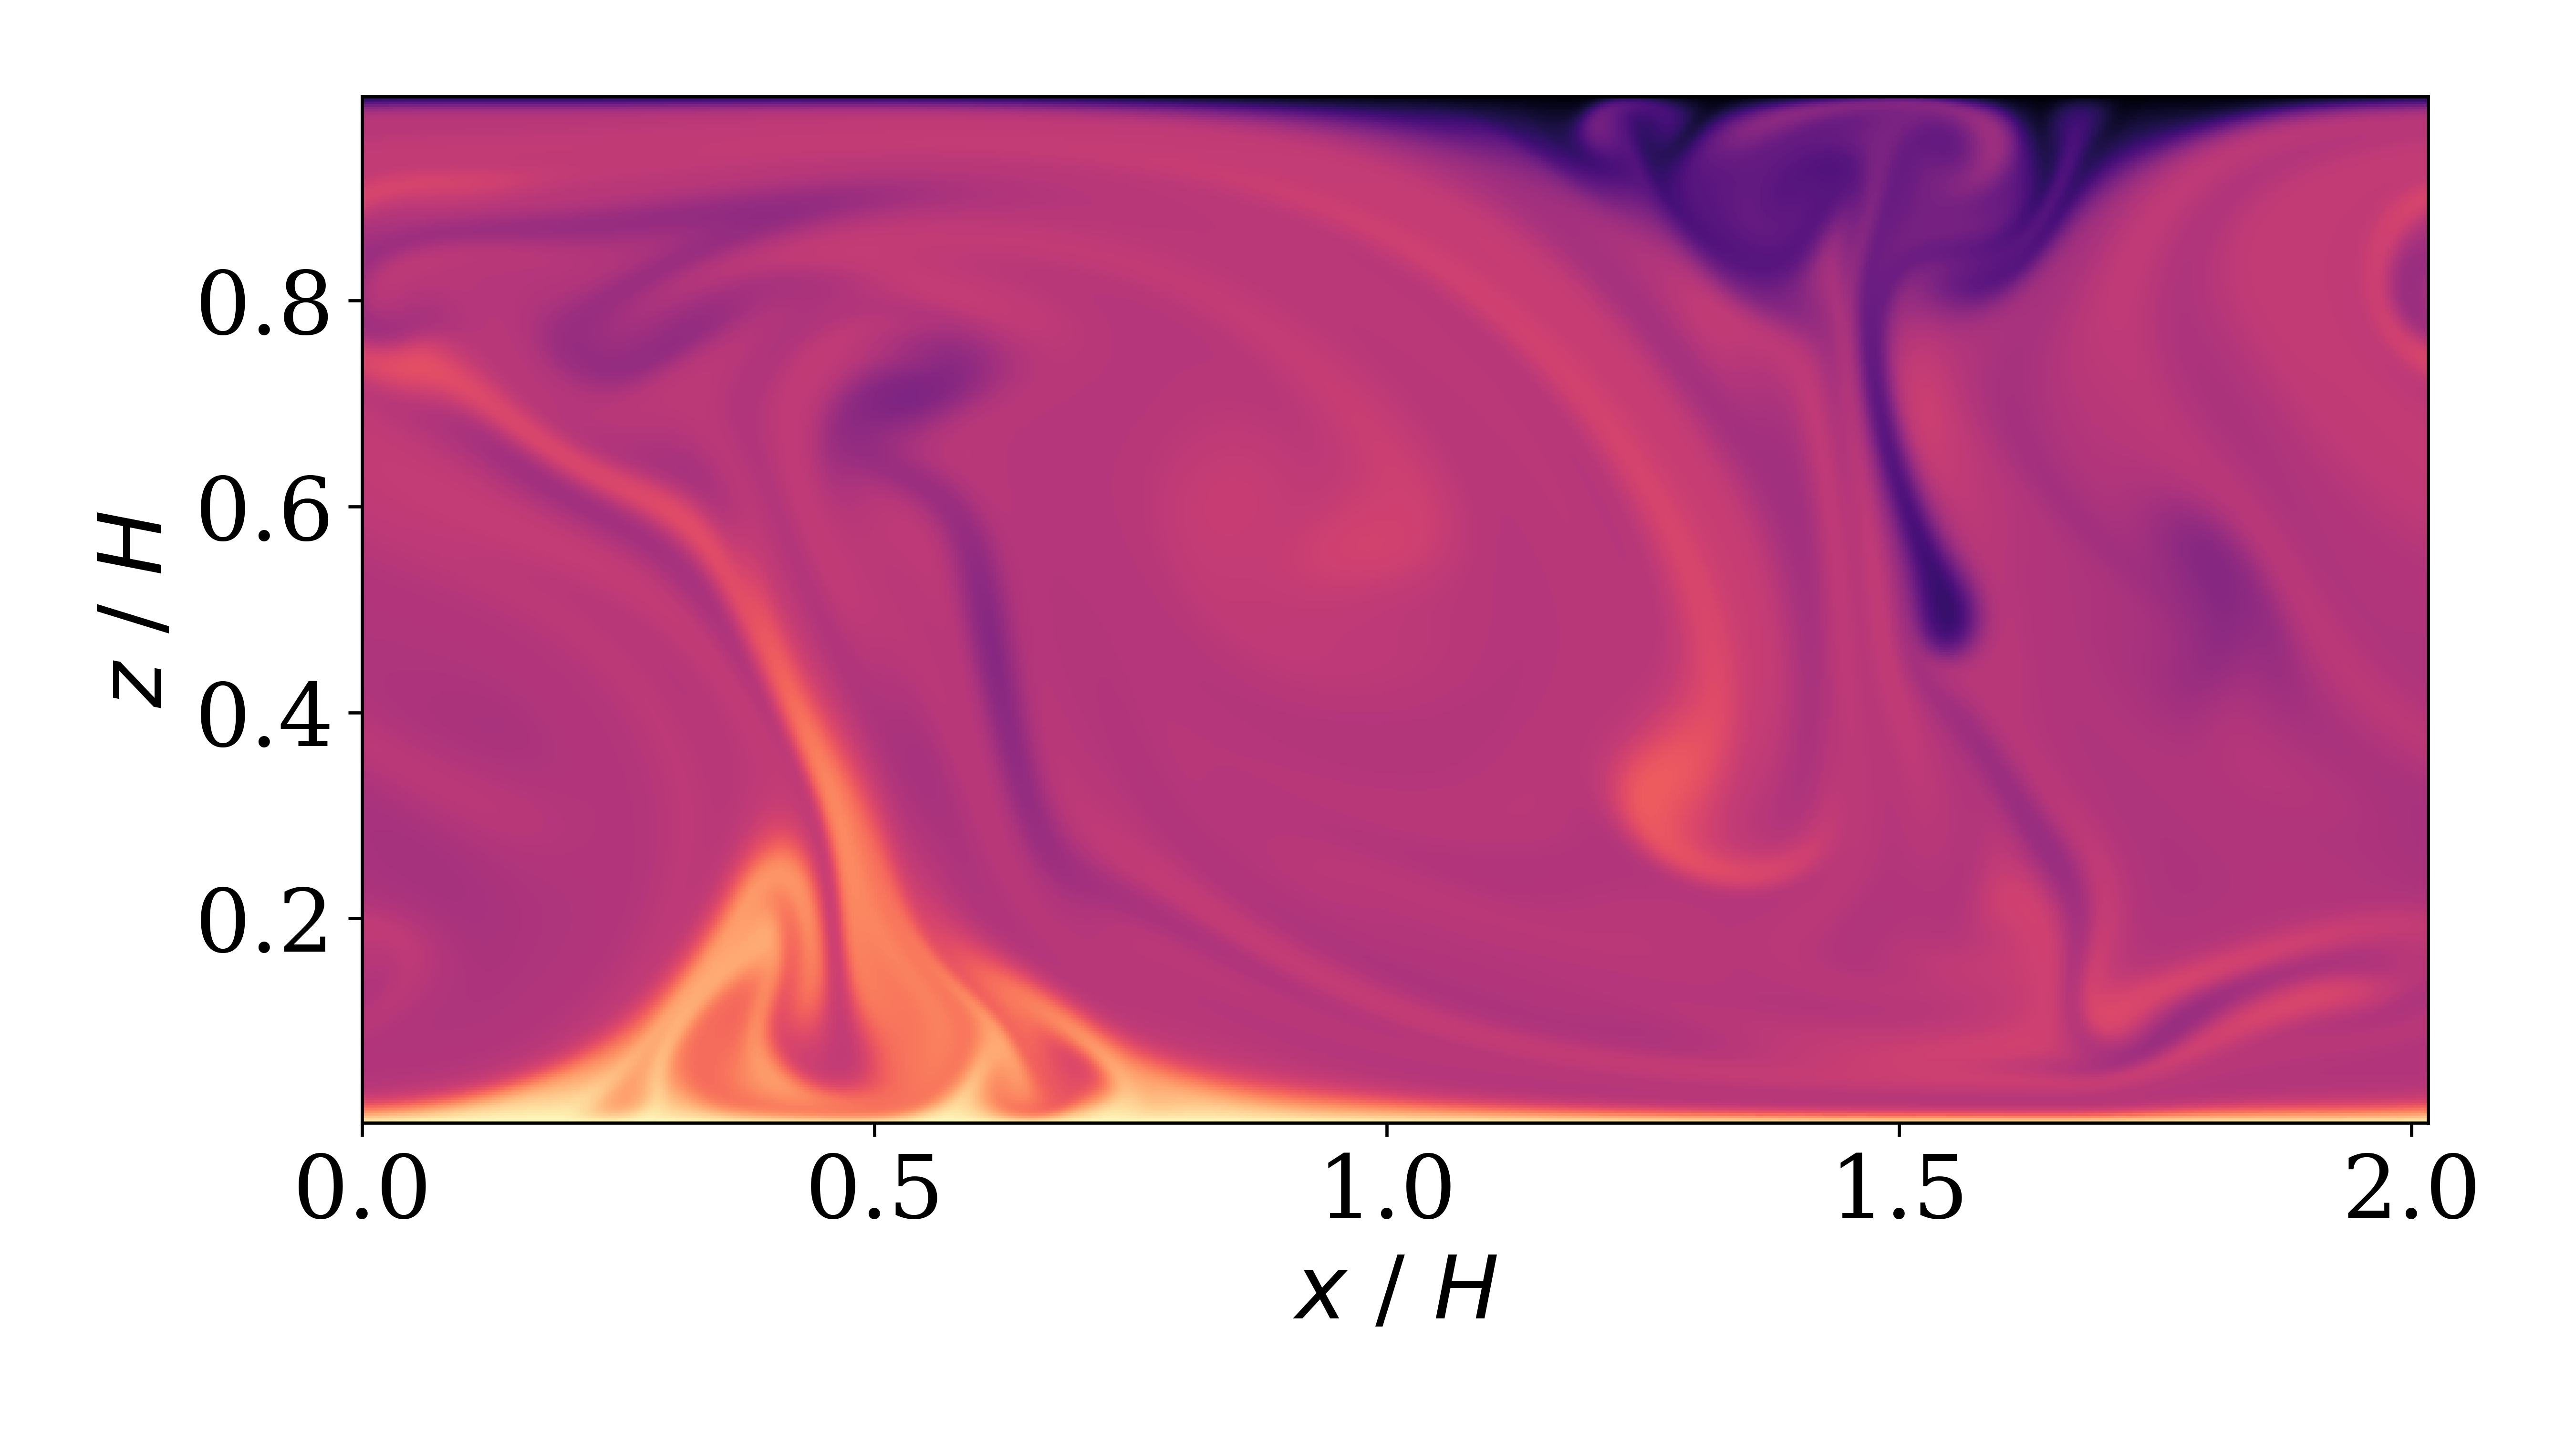
\includegraphics[trim = 0 0 0 25, clip, width=\textwidth]{Ra_1e+08_H1_randIC_Y400_X800_buoyancy_600s_cmapMagma.png}
    \end{subfigure}
    \begin{subfigure}{0.49\textwidth}
        \caption{$\Ra \simeq 10^{10}$}
        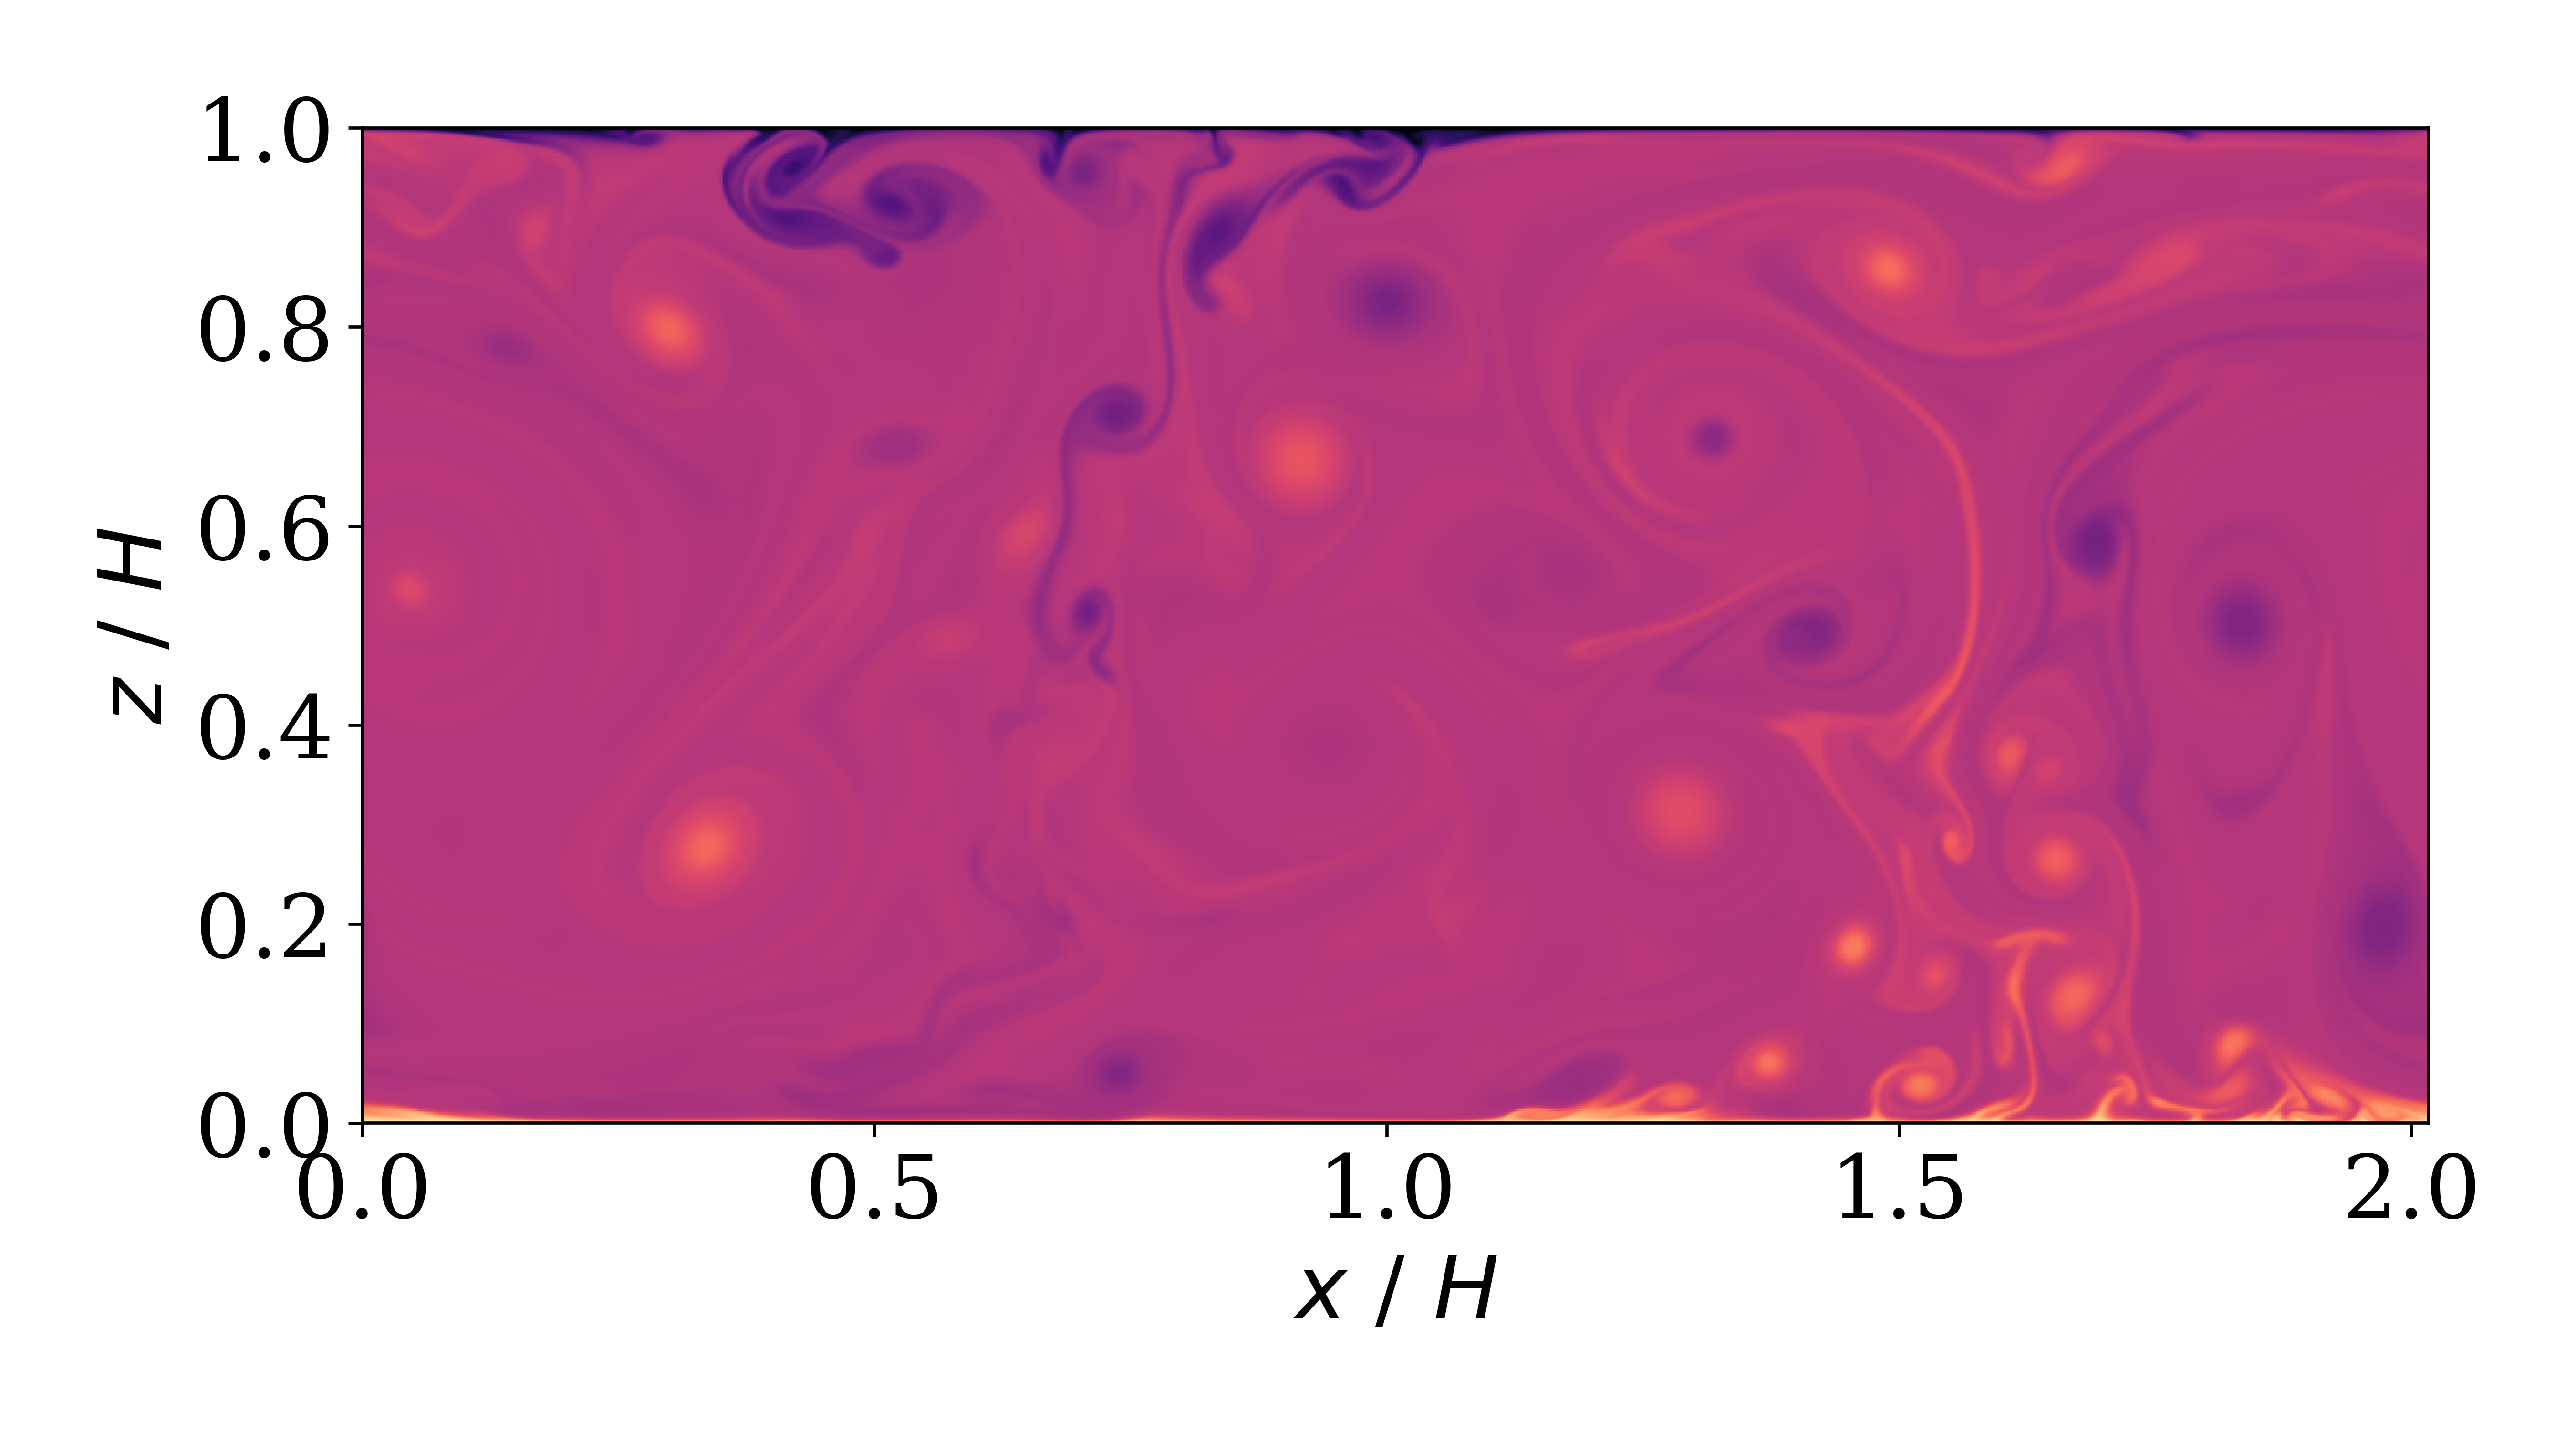
\includegraphics[trim = 0 0 0 25, clip, width=\textwidth]{Ra_1e+10_H1_gradedMesh_2EtaK_buoyancy_900s_cmapMagma.png}
    \end{subfigure}
    \begin{subfigure}[c]{\textwidth}
        \caption*{}
        
\includegraphics[
            trim = 0 0 0 10,
            clip,
            width=0.96\textwidth
        ]{b_colorbar_magma.png}
    \end{subfigure}
    \caption[Example small figure.]{
        Snapshots of buoyancy fields in 2D Rayleigh-B\'{e}nard convection at varying Rayleigh number.
        Partial reproduction of Figure~2.1 of \textcite{phd:Shipley2021}.
    }\label{fig:DNS_RBCexamples}
\end{figure}
\afterpage{%
\clearpage% Flush earlier floats (otherwise order might not be correct)
\begin{landscape}% Landscape page
    \begin{figure}[t!hb]
        \centering
        \begin{subfigure}[t]{\linewidth}
            \caption{Buoyancy, $b / \Delta B$}
            \centering
            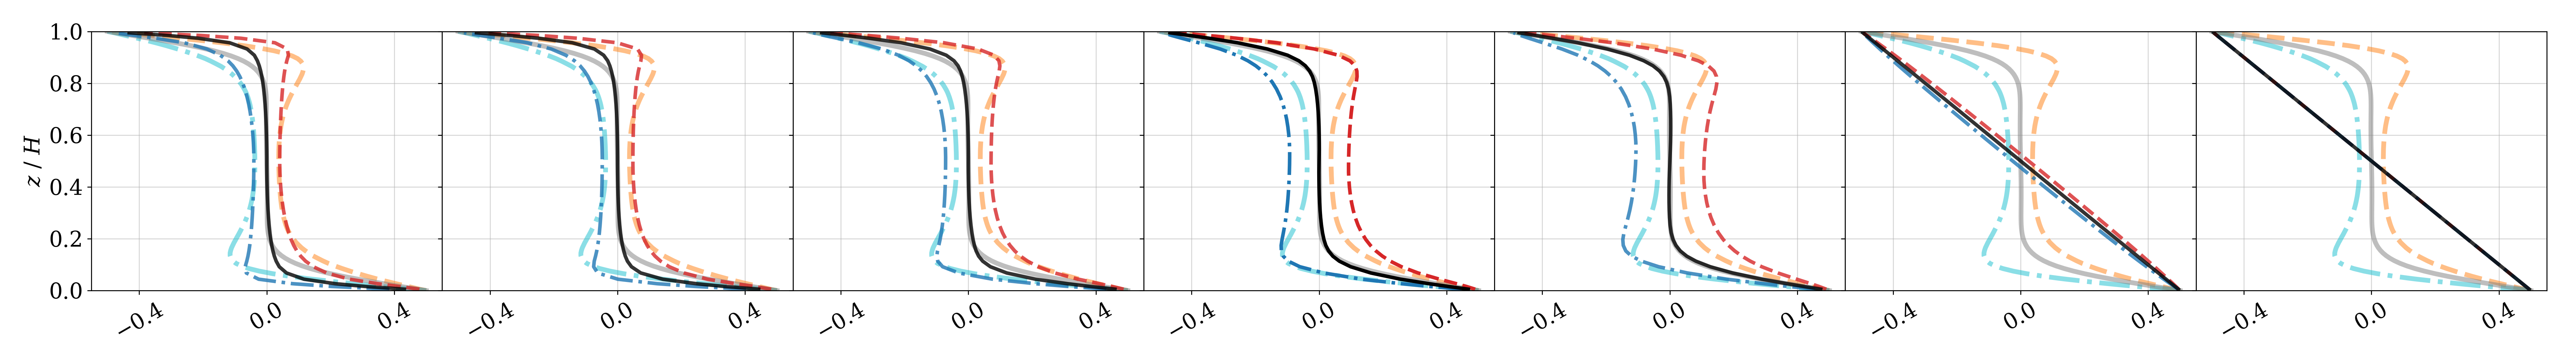
\includegraphics[
                trim = 17 0 18 20,
                clip,
                width=\linewidth
            ]{gammaSensitivity_buoyancyProfiles_separateSubplots.png}
        \end{subfigure}
        \begin{subfigure}[t]{\linewidth}
            \caption{Pressure, $P / (\Delta B\ H)$}
            \centering
            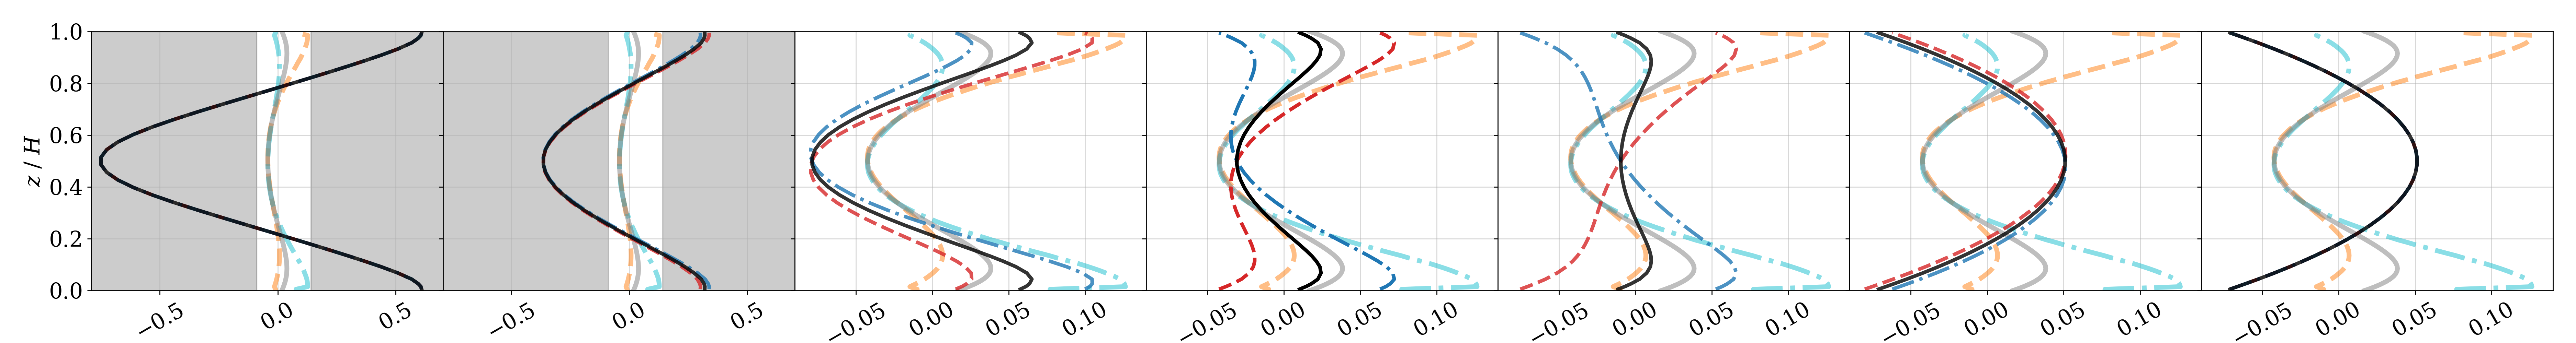
\includegraphics[
                trim = 17 0 18 20,
                clip,
                width=\linewidth
            ]{gammaSensitivity_pressureProfiles_separateSubplots.png}
        \end{subfigure}
        \begin{subfigure}[t]{\linewidth}
            \caption{Vertical velocity, $w / \sqrt{\Delta B\ H}$}
            \centering
            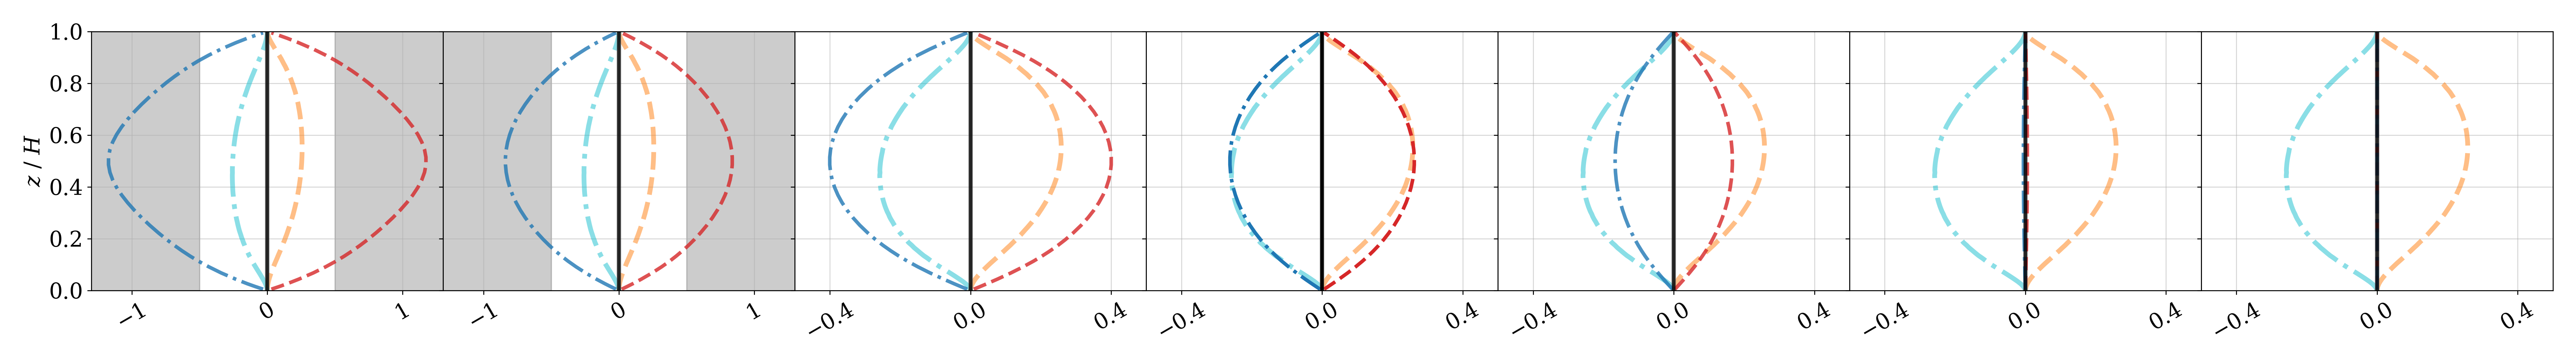
\includegraphics[
                trim = 17 0 18 20,
                clip,
                width=\linewidth
            ]{gammaSensitivity_wProfiles_separateSubplots.png}
        \end{subfigure}
        \begin{subfigure}[t]{\linewidth}
            \centering
            
\includegraphics[
                trim = -30 0 20 0,
                clip,
                width=\linewidth
            ]{gammaSensitivity_gammaLegend.png}
        \end{subfigure}
        \begin{subfigure}[t]{\linewidth}
            \centering
            
\includegraphics[
                trim = -80 0 70 0,
                clip,
                width=\linewidth
            ]{legend_2fProfiles_multiProfileSensitivity.png}
        \end{subfigure}
        \caption[Example large sideways figure.]{
            Two-fluid single-column model of $\Ra = 10^{5}$ Rayleigh-B\'{e}nard convection. 
            Showing sensitivity to the dimensionless closure parameter $\hat{\gamma}_0$, associated with pressure differences between the two fluid partitions, over the range $10^{-1} \leq \hat{\gamma}_0 \leq 10^{1}$.
            Profiles in the limit of asymptotically large ($10^5$) and small ($10^{-5}$) $\hat{\gamma}_0$ are also shown for reference.
            Reproduction of Figure~4.7 in \textcite{phd:Shipley2021}.
        }
        \label{fig:twoFluid_sensitivity_gamma}
    \end{figure}
\end{landscape}
\clearpage
}

\section{Version control; review \& editing}

\subsection{Version control}
I use the \texttt{gitinfo2} package to automatically interface with Git for version control.
Unfortunately this doesn't play nicely with Overleaf, but you can still use the bottom-of-page watermarks to include useful version information manually.
The setup for this is under \texttt{VERSION CONTROL} in the master file \texttt{book\_MWE.tex}.
For ``final'' versions of the document, you can stop the watermarks from appearing by removing the ``\texttt{mark}'' option from the package include statement.

\subsection{Reviewing \& editing}
I have added some simple review \& editing commands that allow text to be added, removed, and edited while retaining the original text and highlighting the changes made (I found this very useful when doing my thesis corrections\dots).
The action of these commands is defined by the truth value of the \texttt{draft} Boolean; this is currently set to \textbf{\texttt{true}} under the heading \texttt{TEXT TO ONLY APPEAR IN DRAFTS} in the master document.
The following lists summarize the use of the commands:

\noindent Verbatim code:
\begin{verbatim}
\begin{itemize}
    \item[\texttt{add}:] \add{
        Here is some new text I have added to the document.
    }
    \item[\texttt{edit}:] \edit{
        Here is some old text I have deleted from the document.
    }{
        Here is some new text I have added to the document.
    }
    \item[\texttt{delete}:] \delete{
        Here is some old text I have deleted from the document.
    }
    \item[\texttt{todonote}:] \todonote{
        Here is a note-to-self for something I still need to do!
    }
\end{itemize}
\end{verbatim}

\noindent Draft true: 
{\drafttrue
\begin{itemize}
    \item[\texttt{add}:] \add{
        Here is some new text I have added to the document.
    }
    \item[\texttt{edit}:] \edit{
        Here is some old text I have deleted from the document.
    }{
        Here is some new text I have added to the document.
    }
    \item[\texttt{delete}:] \delete{
        Here is some old text I have deleted from the document.
    }
    \item[\texttt{todonote}:] \todonote{
        Here is a note-to-self for something I still need to do!
    }
\end{itemize}
}

\noindent Draft false: 
{\draftfalse
\begin{itemize}
    \item[\texttt{add}:] \add{
        Here is some new text I have added to the document.
    }
    \item[\texttt{edit}:] \edit{
        Here is some old text I have deleted from the document.
    }{
        Here is some new text I have added to the document.
    }
    \item[\texttt{delete}:] \delete{
        Here is some old text I have deleted from the document.
    }
    \item[\texttt{todonote}:] \todonote{
        Here is a note-to-self for something I still need to do!
    }
\end{itemize}
}

\section{Referencing}\label{sec:referencing}

The \texttt{hyperref} package is included, such that all citations, back references, and cross-references are hyperlinks.
I prefer hyperlinks to not be coloured, as I found this ends up very messy (and is also easily confused with colour-based annotations).

\subsection{Cross-referencing}
The \verb!cleveref! package gives nice automatic typesetting of cross-references (basically meaning that you don't need to manually type out Chapter, Section, Equation, Figure etc. every time).
This also ensures consistency --- no need to check that you've capitalized ``Figure'' everywhere, or that you've never abbreviated ``Equation''.
Examples: \cref{sec:referencing}; \cref{eq:filter_commutation}; \cref{def:linearFiltering}; \cref{app:additionalThingsToSay}; \cref{fig:twoFluid_sensitivity_gamma}; \cref{tab:solverDetails}.
Note that I like my reference labels to be capitalized and non-abbreviated, but these preferences can easily be changed in the package include statement.

\subsection{Citations and bibliography}
I use \verb!biblatex! exclusively for my bibliography and citations, as I find it far more customizable than either \verb!bibtex! or \verb!natbib!.
Unfortunately this means that many of my setup choices may not port naturally to other choices of bibliography package.

My \verb!biblatex! setup is found under the \texttt{BIBLIOGRAPHY} heading in \texttt{dansBookMacro}.
As standard, this setup excludes the day, month, url, eprint, and isbn fields from bibliography entries (to reduce clutter), and reduces the font size to \verb!small! (the same as figure \& table captions).
The necessary commands to change this part of the setup are hopefully quite self-explanatory.
Here is a brief description of what some of the more opaque options do:
\begin{itemize}
    \item \verb!backref=true! adds references in the bibliography to the page(s) where the reference was cited in the text.
    I also redefined the wording used for the back-references to say ``cit. on p.'' rather than the lengthier ``cited on page''.
    See the \nameref{bibliography} for examples of the backreferences in action.
    \item \verb!style=authoryear-comp! is author-year citation style, with the additional specification that an author's name is only printed once when multiple references passed to the same \verb!\cite! command share the same author.
    I use this because I think it looks cleaner.
    \item \verb!maxcitenames=2! means that a citation will be printed as ``First Author et al.'' if there are more than two authors (rather than the default three).
    \item \verb!uniquelist=false! means that references with differing name lists but identical \textit{truncated} name lists will always be cited as ``First Author et al.''
    Citations with different years are automatically disambiguated by the year (e.g. \cite{ar:SiebesmaEtAl2003}, \cite{ar:SiebesmaEtAl2007}), while citations with the same year have a, b etc. appended to the year (e.g. \cite{ar:GuEtAl2020_JAS}, \cite{ar:GuEtAl2020_GRL}).
    \item \verb!uniquename=init! means that references where authors in the truncated name list share a surname are disambiguated by also providing their initials (e.g. \cite{ar:Malkus1954a}, \cite{ar:RiehlMalkus1958}).
    \item \verb!sorting=nyt! means that references in the bibliography are sorted according to name, then year, then title.
    \item \verb!giveninits=true! means that only the initials of given names are printed in the bibliography, rather than full given names.
    For example, Dan~Shipley will always appear as D.~Shipley in the references.
\end{itemize}

Although it is not an option passed to \verb!biblatex!, I also document here how I enforce correct alphabetical sorting of the names of organizations (for instance The OpenFOAM Foundation should appear as ``The OpenFOAM Foundation'' in a bibliography, but be sorted under ``OpenFOAM'', \textit{not} under ``The''.
This is achieved by defining the \verb!\noopsort! command in the preamble of your \verb!.bib! file:
\begin{verbatim}
    @preamble{ "\providecommand{\noopsort}[1]{} " }
\end{verbatim}
followed by providing the command with the word you wish to sort on as its argument in the \verb!author! field of any relevant bibliography entry.
For instance:
\begin{verbatim}
    @misc{misc:OpenFOAMUserGuide_v7,
        title = {OpenFOAM v7 User Guide},
        author = {{\noopsort{OpenFOAM}The OpenFOAM Foundation}},
        url = {https://cfd.direct/openfoam/user-guide-v7},
        urldate = {2023-02-24},
        year = {2019}
    }
\end{verbatim}

To give an idea of how this setup typesets citations and references, here are some citations to publications of various flavours: \textcite{bk:AchesonElementaryFD,ch:Kasahara2001,ch:BoisKubicki2002,talk:Doering2021MSRI,report:Behrens2009,misc:OpenFOAMUserGuide_v7}.

\subsection{URLs}
URLs are handled by the \verb!xurl! package, which inserts line breaks in sensible places in long URLs.

Example long URL with line break: \url{https://research.reading.ac.uk/meteorology/people/dan-shipley/}

\section{Maths}
Because I'm quite picky about maths typesetting, I created a separate macro for that (\texttt{dansMathsSetup}) which is automatically included in \texttt{dansBookMacro}.
As well as including definitions for things I use a lot that don't currently have associated \LaTeX\ shortcuts, I have re-defined several standard commands that I didn't like the look of. 
A non-exhaustive list follows:
\begin{itemize}
    \item various dimensionless numbers used in fluid dynamics, e.g. \verb!\Re, \Ra, \Ro! gives $\Re, \Ra, \Ro$; 
    \item material derivative operator, \verb!\Dv*{}{t}!: $\Dv*{}{t}$; 
    \item angle-bracket filtering operator,  \verb!\filter{\varphi}!: $\filter{\varphi}$;
    \item resolved part of a flow variable, \verb!\resolved{\varphi}!: $\resolved{\varphi}$; 
    \item subfilter part of a flow variable, \verb!\subfilter{\varphi}!: $\subfilter{\varphi}$;
    \item bold sans-serif tensors, \verb!\tensor{A}!: $\tensor{A}$;
    \item tensor transpose,  \verb!\tensor{A}\trans!: $\tensor{A}\trans$;
    \item trace operator, \verb!\trace{\tensor{A}}!: $\trace{\tensor{A}}$;
    \item double-colon tensor contraction, \verb!\tensor{A}\contract\tensor{B}!: $\tensor{A}\contract\tensor{B}$; 
    \item $d$-dimensional identity tensor,  \verb!\ident[d]!: $\ident[d]$; 
    \item horizontal divergence \verb!\divH{\vec{u}}!: $\divH{\vec{u}}$;
    \item a Laplacian operator that is consistent with $\grad$, \verb!\laplacian{}!: $\laplacian{}$;
    \item Laplacian and divergence operators with tildes/circumflexes, e.g. \verb!\divhat{}!: $\divhat{}$, \verb!\laplaciantilde{}!: $\laplaciantilde{}$;
    \item \verb!\diff{x}!, which generates a nice upright $\diff{x}$ for use in integrals (e.g. $\int f(x) \diff{x}$ vs. $\int f(x) dx$) or standalone as a differential form.
\end{itemize}

In addition to defining math-mode commands, \texttt{dansMathsSetup} includes definitions of some environments useful for maths-heavy texts, such as bespoke Theorem, Definition, Assumption, and Aside environments.

Finally, the \verb!\allowdisplaybreaks! command allows display-mode mathematics to break over a page break --- exceptionally useful if you don't want weird whitespace appearing whenever you have long equations.

\subsection{Examples}
Here are some examples of the what \texttt{dansMathsSetup} allows; take a look at the raw \LaTeX\ to see whether you think my shortcuts and environments might be useful to you.
If not, hopefully a look at the command definitions should show that it is easy to define custom math mode commands that \textit{will} be of use.

\noindent\rule{\textwidth}{0.4pt}

We shall consider a dry Boussinesq fluid governed by the following equation set:
\begin{align}
    \Dv{\vec{u}}{t}
    &=
    b \vec{k}
  - \grad{P}
  + \nu \laplacian{\vec{u}},
    \label{eq:SFBoussinesq_momentum}
    %%%%%%%%%%%%%%%%%%%%%%%%%%%%%%%%%%%%%%%%%%%%%%%%%%%%%%%%%%%%%%%
    \\
    \Dv{b}{t}
    &=
    \kappa\laplacian{b},
    \label{eq:SFBoussinesq_buoyancy}
    %%%%%%%%%%%%%%%%%%%%%%%%%%%%%%%%%%%%%%%%%%%%%%%%%%%%%%%%%%%%%%%
    \\
    \div{\vec{u}}
    &=
    0.
    \label{eq:SFBoussinesq_mass}
    %%%%%%%%%%%%%%%%%%%%%%%%%%%%%%%%%%%%%%%%%%%%%%%%%%%%%%%%%%%%%%%
\end{align}
Here $\vec{u}$ is the velocity field, $b$ is the buoyancy field, $P$ is the pressure field, $\nu$ is the fluid's kinematic viscosity, and $\kappa$ its buoyancy diffusivity.
$\vec{k}$ is a unit vector antiparallel to gravity, i.e. $\vec{k} \coloneqq - \flatfrac{\vec{g}}{\abs{\vec{g}}}$, defining the vertical ($\unit{z}$) direction.
We envisage solving this equation set in the space-time domain $D \times [0,T]$, where $D \subseteq \mathbb{R}^d$ (with $d \in \set{2,3}$), $T \in \mathbb{R}_{>0}$.

For most cases of interest to us, the flow will be turbulent, and so we nondimensionalize the equations in a way that is suitable for studying turbulence; that is, where the inertial forces are much more important than diffusive forces, and where neither the diffusion of momentum nor buoyancy is considered negligible, $\flatfrac{\nu}{\kappa} = \mathcal{O}(1)$.
To do this we perform an isotropic rescaling of the dimensional parameters in the problem:
\begin{align}
    b \to \Delta B\ b, 
    \quad
    \vec{x} \to H \vec{x},
    \quad
    t \to \sqrt{\frac{H}{\Delta B}}\ t,
    \quad
    \vec{u} \to \sqrt{\Delta B \cdot H}\ \vec{u},
    \quad
    P \to \Delta B\ H\ P.
\end{align}
Here $\Delta B \in \mathbb{R}_{>0}$ is a characteristic buoyancy difference across a layer of fluid of depth $H \in \mathbb{R}_{>0}$, i.e. $\Delta B \coloneqq b(z = z_0) - b(z = z_0 + H)$.
Note that this rescaling is only defined for an unstably-stratified flow, since we force $\Delta B \in \mathbb{R}_{>0}$.
The resulting nondimensionalized equation set is:
\begin{align}
    \Dv{\vec{u}}{t}
    &=
    b \vec{k}
  - \grad{P}
  + \sqrt{\frac{\Pr}{\Ra}} \laplacian{\vec{u}},
    \label{eq:SFBoussinesq_momentum_nonDim}
    %%%%%%%%%%%%%%%%%%%%%%%%%%%%%%%%%%%%%%%%%%%%%%%%%%%%%%%%%%%%%%%
    \\
    \Dv{b}{t}
    &=
    \frac{1}{\sqrt{\Ra\Pr}} \laplacian{b},
    \label{eq:SFBoussinesq_buoyancy_nonDim}
    %%%%%%%%%%%%%%%%%%%%%%%%%%%%%%%%%%%%%%%%%%%%%%%%%%%%%%%%%%%%%%%
    \\
    \div{\vec{u}}
    &=
    0.
    \label{eq:SFBoussinesq_mass_nonDim}
    %%%%%%%%%%%%%%%%%%%%%%%%%%%%%%%%%%%%%%%%%%%%%%%%%%%%%%%%%%%%%%%
\end{align}
Comparison with the standard nondimensionalized incompressible Navier-Stokes equations suggests the identification $\Re \sim \sqrt{\flatfrac{\Ra}{\Pr}}$.

The range of dynamically important spatiotemporal scales in a turbulent flow is vast\footnote{
    Scaling like $\eta/\ell \sim \Re^{3/4}$, where $\eta$ is the Kolmogorov microscale, the smallest dynamically important length scale in the flow, and $\ell$ is the characteristic energy injection length scale.
}, and so we must introduce some notion of mode reduction, averaging, or filtering, to make the equations tractable.
With this in mind, we make the following definitions:

\begin{definition}[Linear filtering operation]\label{def:linearFiltering}
    Given flow variables $\varphi, \psi$, and constant $\alpha \in \mathbb{R}$, we define a \textbf{linear filtering operation}, denoted by angle brackets, $\filter{\dots}$, as a formal operation that is \textbf{linear}:
    \begin{align}
        \filter{\varphi + \psi}
        &=
        \filter{\varphi}
      + \filter{\psi}
        \label{eq:filter_linearity}
    \end{align}
    and \textbf{constant-preserving}:
    \begin{align}
        \filter{\alpha\varphi}
        &=
        \alpha\filter{\varphi}.
    \end{align}
    Additionally, it is usually assumed in fluid dynamics that such filters commute with space and time translations, or equivalently that they commute with space and time partial derivatives:
    \begin{align}
        \filter{\pdv{\varphi}{\vec{x}}}
        =
        \pdv{\filter{\varphi}}{\vec{x}},
        \quad
        \filter{\pdv{\varphi}{t}}
        &=
        \pdv{\filter{\varphi}}{t}
        \label{eq:filter_commutation},
    \end{align}
    though one must be careful with this assumption in the vicinity of boundaries.
    Unless otherwise explicitly stated, in this text a ``linear filtering operator'' is linear, constant-preserving, and commutes with space and time translations.
\end{definition}

\begin{aside}
    A Reynolds averaging operator, $\filter{\dots}_\text{R}$, is a special case of a linear filtering operator which satisfies also the following ``Reynolds condition'':
    \begin{align}
        \filter{\varphi\filter{\psi}_\mathrm{R}}_\mathrm{R}
        &=
        \filter{\varphi}_\mathrm{R} \filter{\psi}_\mathrm{R}
        \\
        \implies
        \filter{\filter{\varphi}_\mathrm{R}}_\mathrm{R}
        = 
        \filter{\varphi}_\mathrm{R},
        &\quad
        \filter{
            \filter{\varphi}_\mathrm{R}
          - \varphi
        }_\mathrm{R}
        =
        0,
    \end{align}
    that is, the Reynolds averaging operator projects the flow onto a sub-space of the solution phase space which is invariant under whatever group action the operator is averaging along.
    As a specific example, if the average is a time average, the corresponding Reynolds operator projects onto a time-invariant --- or ``stationary'' --- sub-space (and so, Reynolds-averaged flows constructed based on time averages \textit{cannot} have time dependence --- see e.g. \cite{bk:TennekesLumleyTurb}, p.28).
    Similar must be true if the average is a spatial average: the corresponding Reynolds operator then projects onto a spatially-invariant --- or ``homogeneous'' --- sub-space, meaning that the spatially Reynolds-averaged flow cannot have any spatial dependence.
    
    Again, note that a Reynolds averaging operator need not \textit{necessarily} commute with space and time translations, and therefore space/time partial derivatives, though Reynolds operators in fluid dynamics are usually assumed to commute with either Eulerian or Lagrangian translations.
\end{aside}

\begin{definition}[Spatial filter]\label{def:spatialFilter}
    For a flow variable $\varphi(\vec{x},t)$ we define the operation of \textbf{(integral) spatial filtering} by:
    \begin{align}
        \filter{\varphi}_g
        &\coloneqq
        \int_{\mathbb{R}^d}
            g(\vec{x} - \vec{x}^\prime; \vec{\delta})
            \varphi(\vec{x}^\prime, t)
        \diff[d]{\vec{x}^\prime},
        \label{eq:spatialFilterDefinition}
    \end{align}
    where $g(\vec{x} - \vec{x}^\prime; \vec{\delta})$ is a \textbf{filter kernel} satisfying the normalization condition:
    \begin{align}
        \int_{\mathbb{R}^d}
            g(\vec{x} - \vec{x}^\prime; \vec{\delta})
        \diff[d]{\vec{x}^\prime}
        &=
        1.
    \end{align}
    $\filter{\dots}_g$ is read as ``filtering with respect to the kernel $g$''.
    We also require that the filter kernel guarantees the following properties \parencite{bk:BerselliEtAlLES}:
    \begin{align}
        \lim_{\abs{\vec{\delta}} \to 0} \filter{\varphi}
        =
        \varphi,
        \\
        \norm{\filter{\varphi}}
        \leq
        C \norm{\varphi}
        \quad 
        \text{(uniformly in $\abs{\vec{\delta}}$)},
    \end{align}
    which can be interpreted simply as requiring that it is ``well-behaved''.
\end{definition}
    
\begin{aside}
    Such a filter is guaranteed to be linear, although it will not in general commute with space- or time-translations due to the presence of boundaries, and the possibility of the filter width having space- or time-dependence.
    See \textcite{ar:FurebyTabor1997} for details.

    One way to extend spatial filtering to bounded domains in a ``nice'' way is to identify the filter kernel $g(\vec{x} - \vec{x}^\prime; \vec{\delta})$ with the Green's function of a (linear) partial differential equation relating the filtered and unfiltered fields.
    For infinite domains, the integral and differential filter representations produce identical results; however, for bounded domains, the PDE defining the differential filter must be supplemented with appropriate boundary (and initial) conditions which cause the representations to differ in the vicinity of boundaries.
    This allows the differential representation to remain commutative with space- and time-translations even on bounded domains.
\end{aside}

\begin{definition}[``Resolved'' and ``subfilter'' variables: incompressible case]\label{def:resolvedVariables}
    For a variable $\varphi$, and filtering operation $\langle\dots\rangle_g$, we define the \textbf{resolved part of $\varphi$} by:
    \begin{equation}
        \resolved{\varphi}
        \coloneqq
        \left\langle
            \varphi
        \right\rangle_g.
        \label{eq:resolvedVarDefinition}
    \end{equation}
    The \textbf{subfilter part of $\varphi$} is then defined by:
    \begin{equation}
        \subfilter{\varphi}
        \coloneqq
        \varphi - \resolved{\varphi}.
        \label{eq:subfilterVarDefinition}
    \end{equation}
    
    Together these definitions amount to a generalization of the so-called ``Reynolds decomposition'' of a flow into its mean (``resolved'') and fluctuating/eddy (``subfilter'') components.
    Given a flow variable $\varphi$ and a linear filtering operation $\filter[g]{\dots}$, this decomposition is unique.
    However note that a) different filtering operations can give rise to \textit{very} different resolved flows; b) a resolved flow is generally consistent with many subfilter flows.
\end{definition}

The linear filtering operations defined in Definition~\ref{def:linearFiltering} are \textit{very} general, and do not inherently include any notion of scale-selection or mode-reduction.
It is only with more specific constructions (like the integral filters of Definition~\ref{def:spatialFilter}) that such notions are introduced.
Since we shall be studying turbulence, we later intend to specify some sort of scale-selection; henceforth our language will reflect that philosophical choice, even though the equations presented remain valid for an arbitrary linear filter.

Therefore let us apply a linear filter to the governing Boussinesq equations~\eqref{eq:SFBoussinesq_momentum_nonDim}--\eqref{eq:SFBoussinesq_mass_nonDim}:
\begin{align}
    \pdv{\resolved{\vec{u}}}{t}
  + \div(
        \resolved{\vec{u}} \otimes \resolved{\vec{u}}
    )
    &=
    \resolved{b} \vec{k}
  - \grad{\resolved{P}}
  + \sqrt{\frac{\Pr}{\Ra}}\laplacian{\resolved{\vec{u}}}
  - \div{ s(\vec{u},\vec{u}) },
    \label{eq:SFBoussinesq_momentum_filtered}
    %%%%%%%%%%%%%%%%%%%%%%%%%%%%%%%%%%%%%%%%%%%%%%%%%%%%%%%%%%%%%%%
    \\
    \pdv{\resolved{b}}{t}
  + \div{\resolved{\vec{u}}\resolved{b}}
    &=
    \frac{1}{\sqrt{\Ra\ \Pr}}\laplacian{\resolved{b}}
  - \div{ s(\vec{u},b) },
    \label{eq:SFBoussinesq_buoyancy_filtered}
    %%%%%%%%%%%%%%%%%%%%%%%%%%%%%%%%%%%%%%%%%%%%%%%%%%%%%%%%%%%%%%%
    \\
    \div{\resolved{\vec{u}}}
    &=
    0.
    \label{eq:SFBoussinesq_mass_filtered}
    %%%%%%%%%%%%%%%%%%%%%%%%%%%%%%%%%%%%%%%%%%%%%%%%%%%%%%%%%%%%%%%
\end{align}
The terms requiring closure are the subfilter fluxes of momentum, $s(\vec{u},\vec{u}) \coloneqq \resolved{\left(\vec{u}\otimes\vec{u}\right)} - \resolved{\vec{u}}\otimes\resolved{\vec{u}}$, and buoyancy, $s(\vec{u},b) \coloneqq \resolved{\left(\vec{u}b\right)} - \resolved{\vec{u}}\resolved{b}$.
If the linear filtering operator is a Reynolds operator, the expressions for the subfilter fluxes simplify:
\begin{align}
    s(a,b)
    &\coloneqq
    \resolved{(ab)}
  - \resolved{a}\resolved{b}
    \nonumber
    \\
    &=
    \resolved{
        \left(\resolved{a}\resolved{b}\right)
      + \left(\resolved{a}\subfilter{b}\right)
      + \left(\subfilter{a}\resolved{b}\right)
      + \left(\subfilter{a}\subfilter{b}\right)
    }
  - \resolved{a}\resolved{b}
    \nonumber
    \\
    \implies
    s_\mathrm{R}(a,b)
    &=
    \reynolds{\reynolds{a}\reynolds{b}}
  + \reynolds{\reynolds{a}\subfilter{b}}
  + \reynolds{\subfilter{a}\reynolds{b}}
  + \reynolds{\subfilter{a}\subfilter{b}}
  - \reynolds{a}\reynolds{b}
    \\
    &=
    \reynolds{a}\reynolds{b}
  + \reynolds{a}\reynolds{\subfilter{b}}
  + \reynolds{\subfilter{a}}\reynolds{b}
  + \reynolds{\subfilter{a}\subfilter{b}}
  - \reynolds{a}\reynolds{b}
    \\
    &=
    \reynolds{\subfilter{a}\subfilter{b}}.
\end{align}
Using the more common notation $\reynolds{\dots} \to \overline{\left(\dots\right)}$ and $\subfilter{\varphi} \to \varphi^\prime$, this can be seen to match the usual expression $\overline{a^\prime b^\prime}$ for the ``eddy covariance'' between $a$ and $b$.
\noindent\rule{\textwidth}{0.4pt}

\section{Thanks}

My thanks to everyone who has commented on or suggested changes to this template, as well as those whose ideas I've borrowed/stolen\dots
You've made it much better than it would otherwise have been!
A particular shout out to: Hilary Weller, Peter Clark, Harriet Turner.

Thank you also to anyone who uses the template; I hope you find it useful.

If you have any comments, error reports, or suggestions for improvement, please email me at \href{mailto:daniel.shipley@reading.ac.uk}{daniel.shipley@reading.ac.uk}.

\cleardoublepage

\include{book/chapters/aSecondChapter}

% appendices
\begin{appendices}
    \renewcommand{\chaptername}{Appendix}
    \chapter{Additional things I didn't have space to say in the main text}\label{app:additionalThingsToSay}

\blindmathpaper

\cleardoublepage
\end{appendices}

% back matter
\backmatter
\setcounter{chapter}{-1} % reset chapter counter so number doesn't appear in header
\pagestyle{frontAndBack}
\printbibliography[heading=bibintoc,title={Bibliography\label{bibliography}}]

\end{document}